\subsection{Algorithm sketch}
\setlength{\unitlength}{0.8cm}
  \begin{figure}[H]
  \centering
  \begin{minipage}[!hp]{0.45\linewidth}
  \centering
    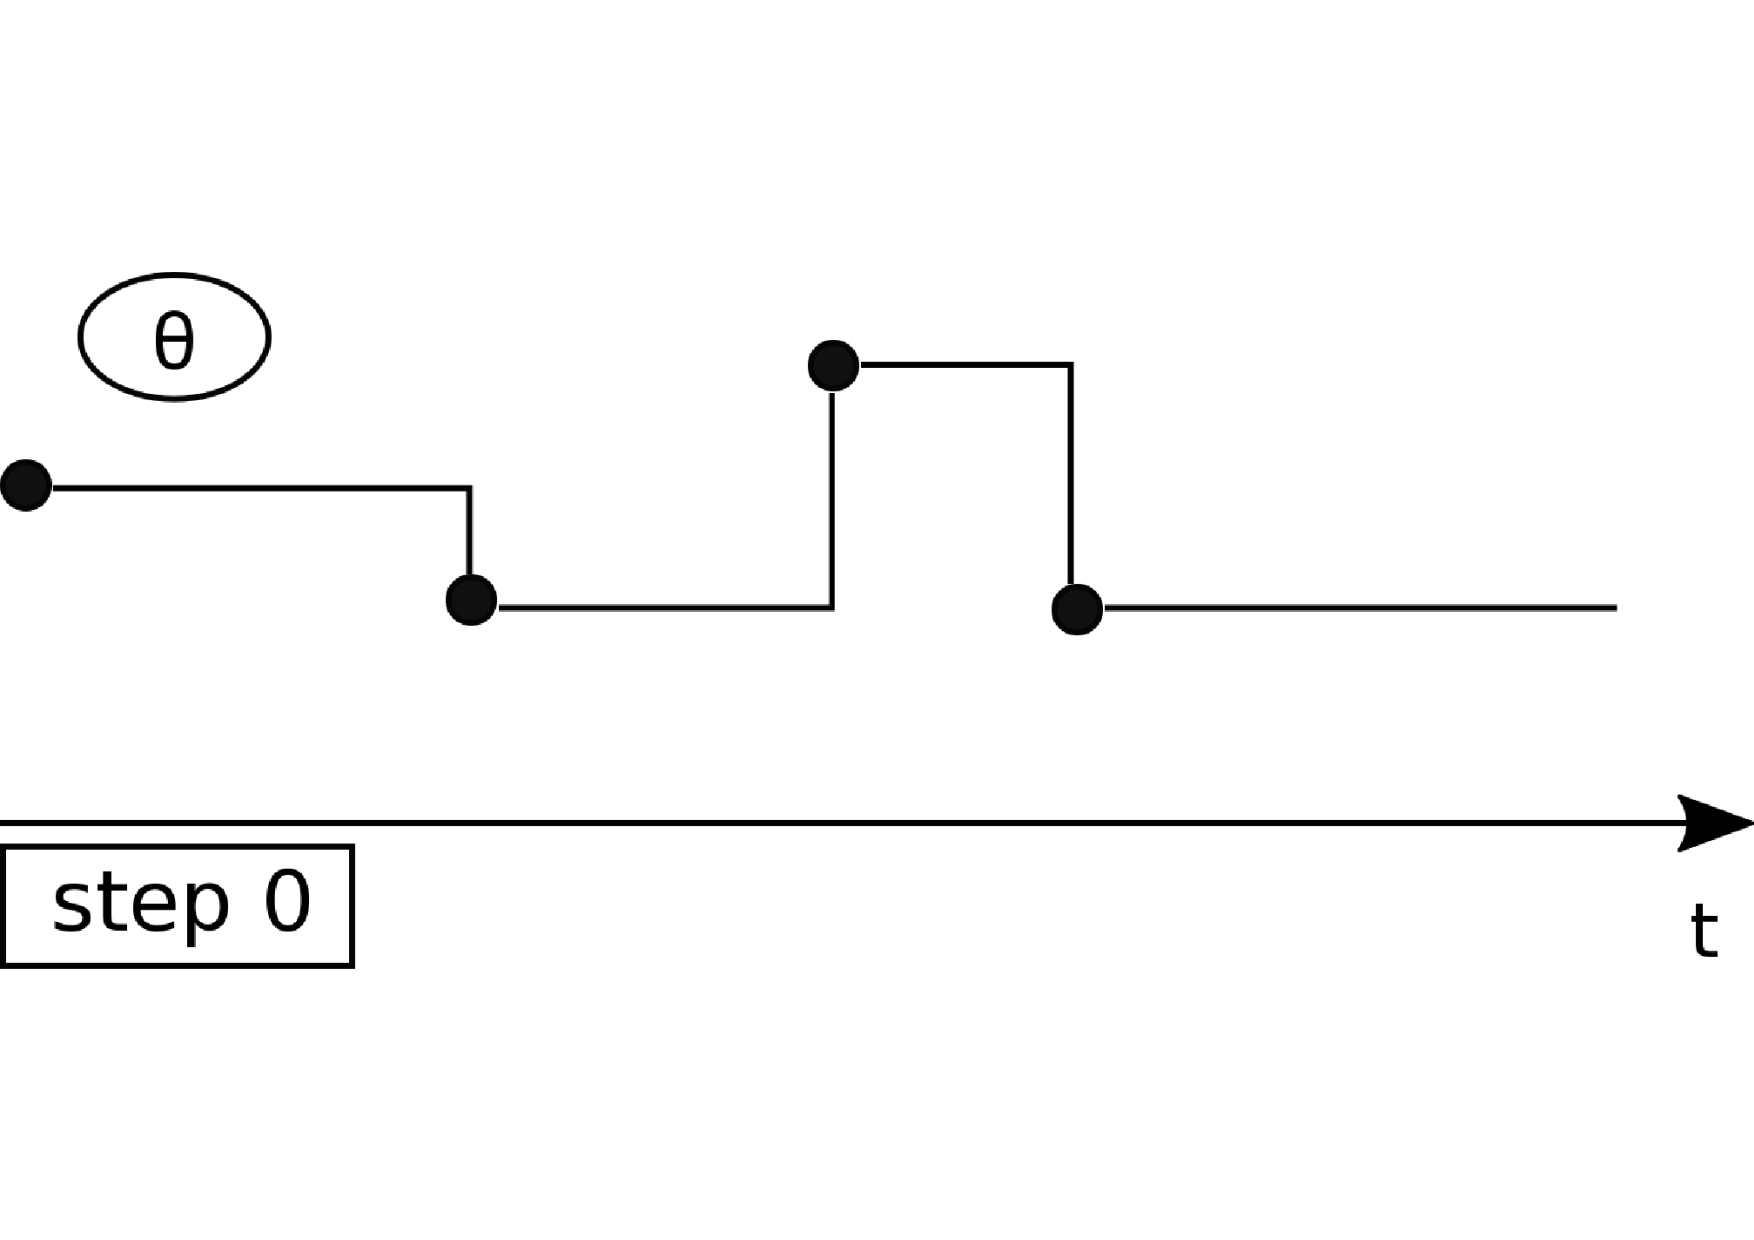
\includegraphics [width=0.70\textwidth, angle=0]{figs/plotn0.pdf}
      \end{minipage}
  \begin{minipage}[!hp]{0.45\linewidth}
  \centering
    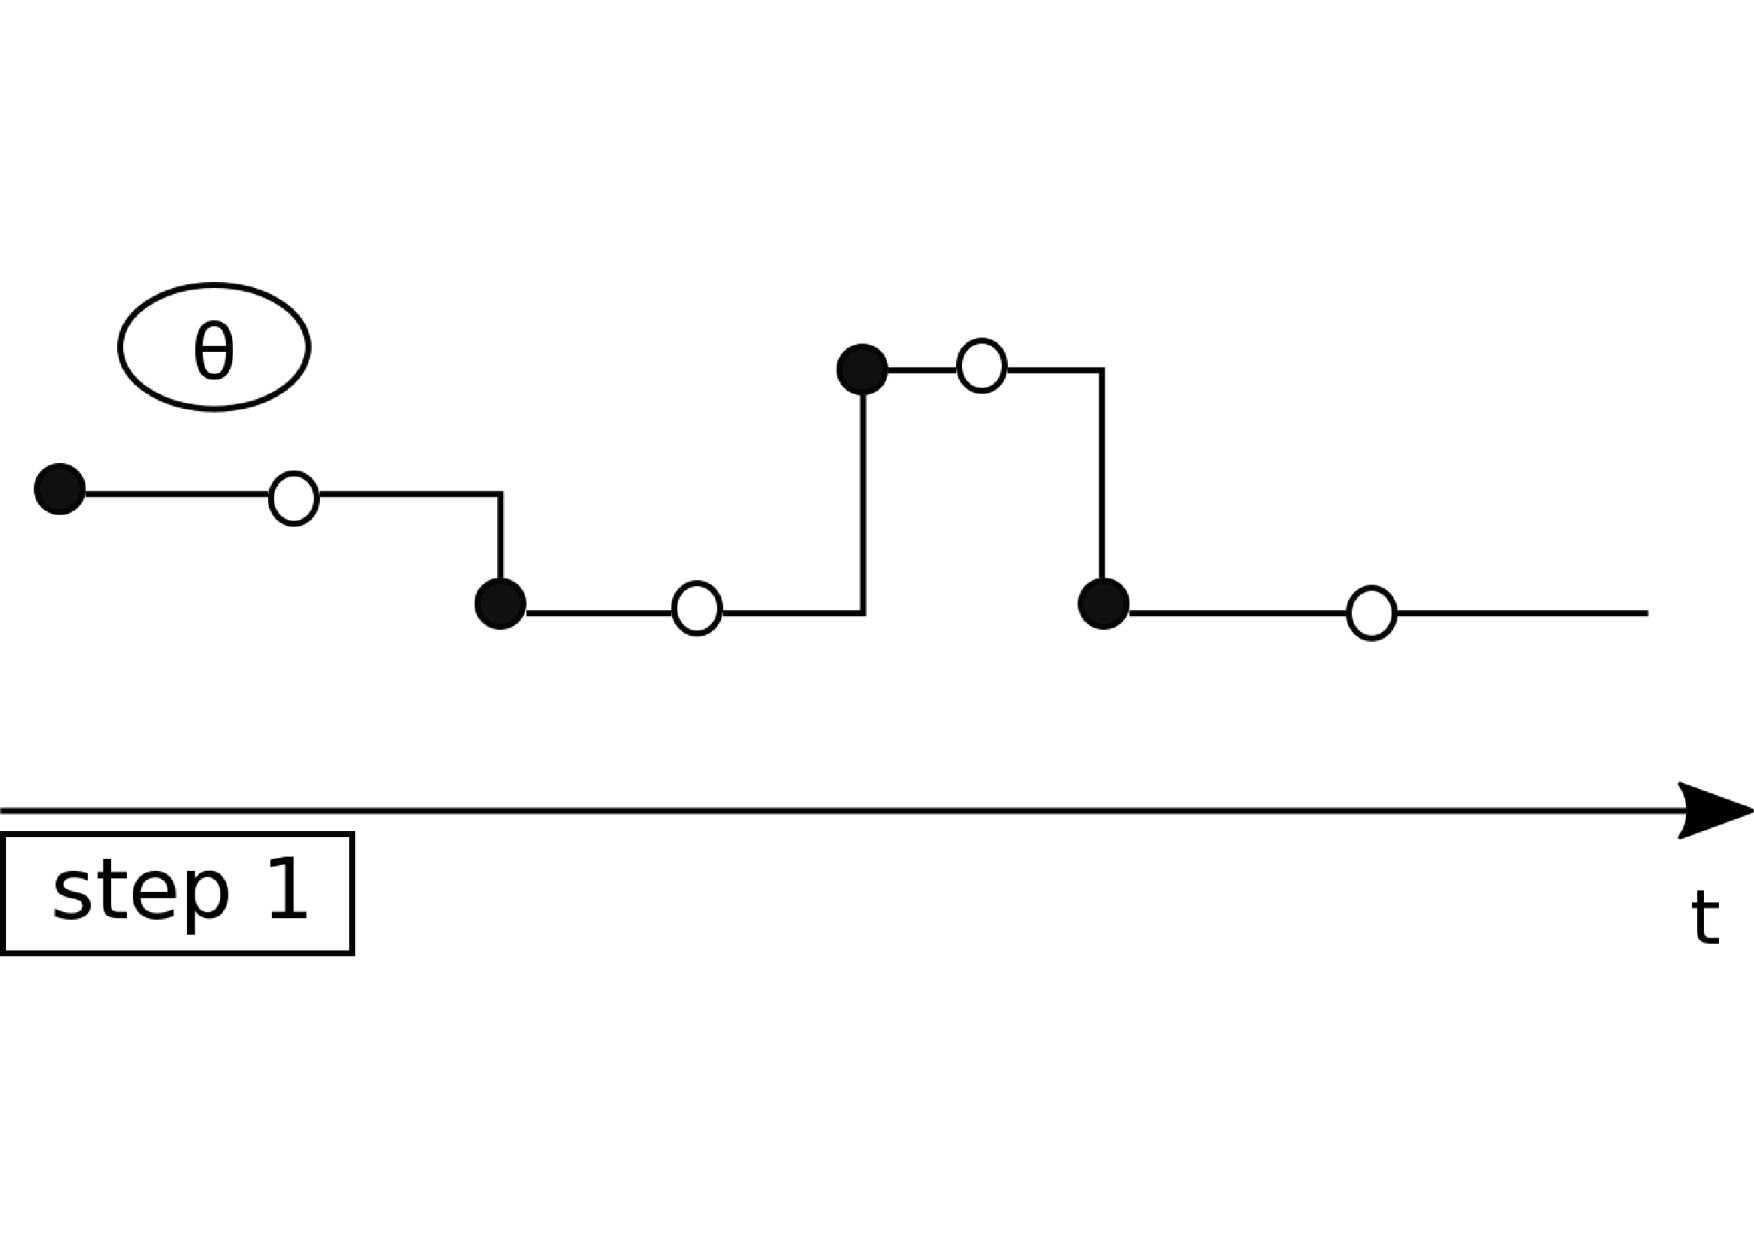
\includegraphics [width=0.70\textwidth, angle=0]{figs/plotn1.pdf}
    \vspace{-0 in}
  \end{minipage}
  \begin{minipage}[!hp]{0.45\linewidth}
  \centering
    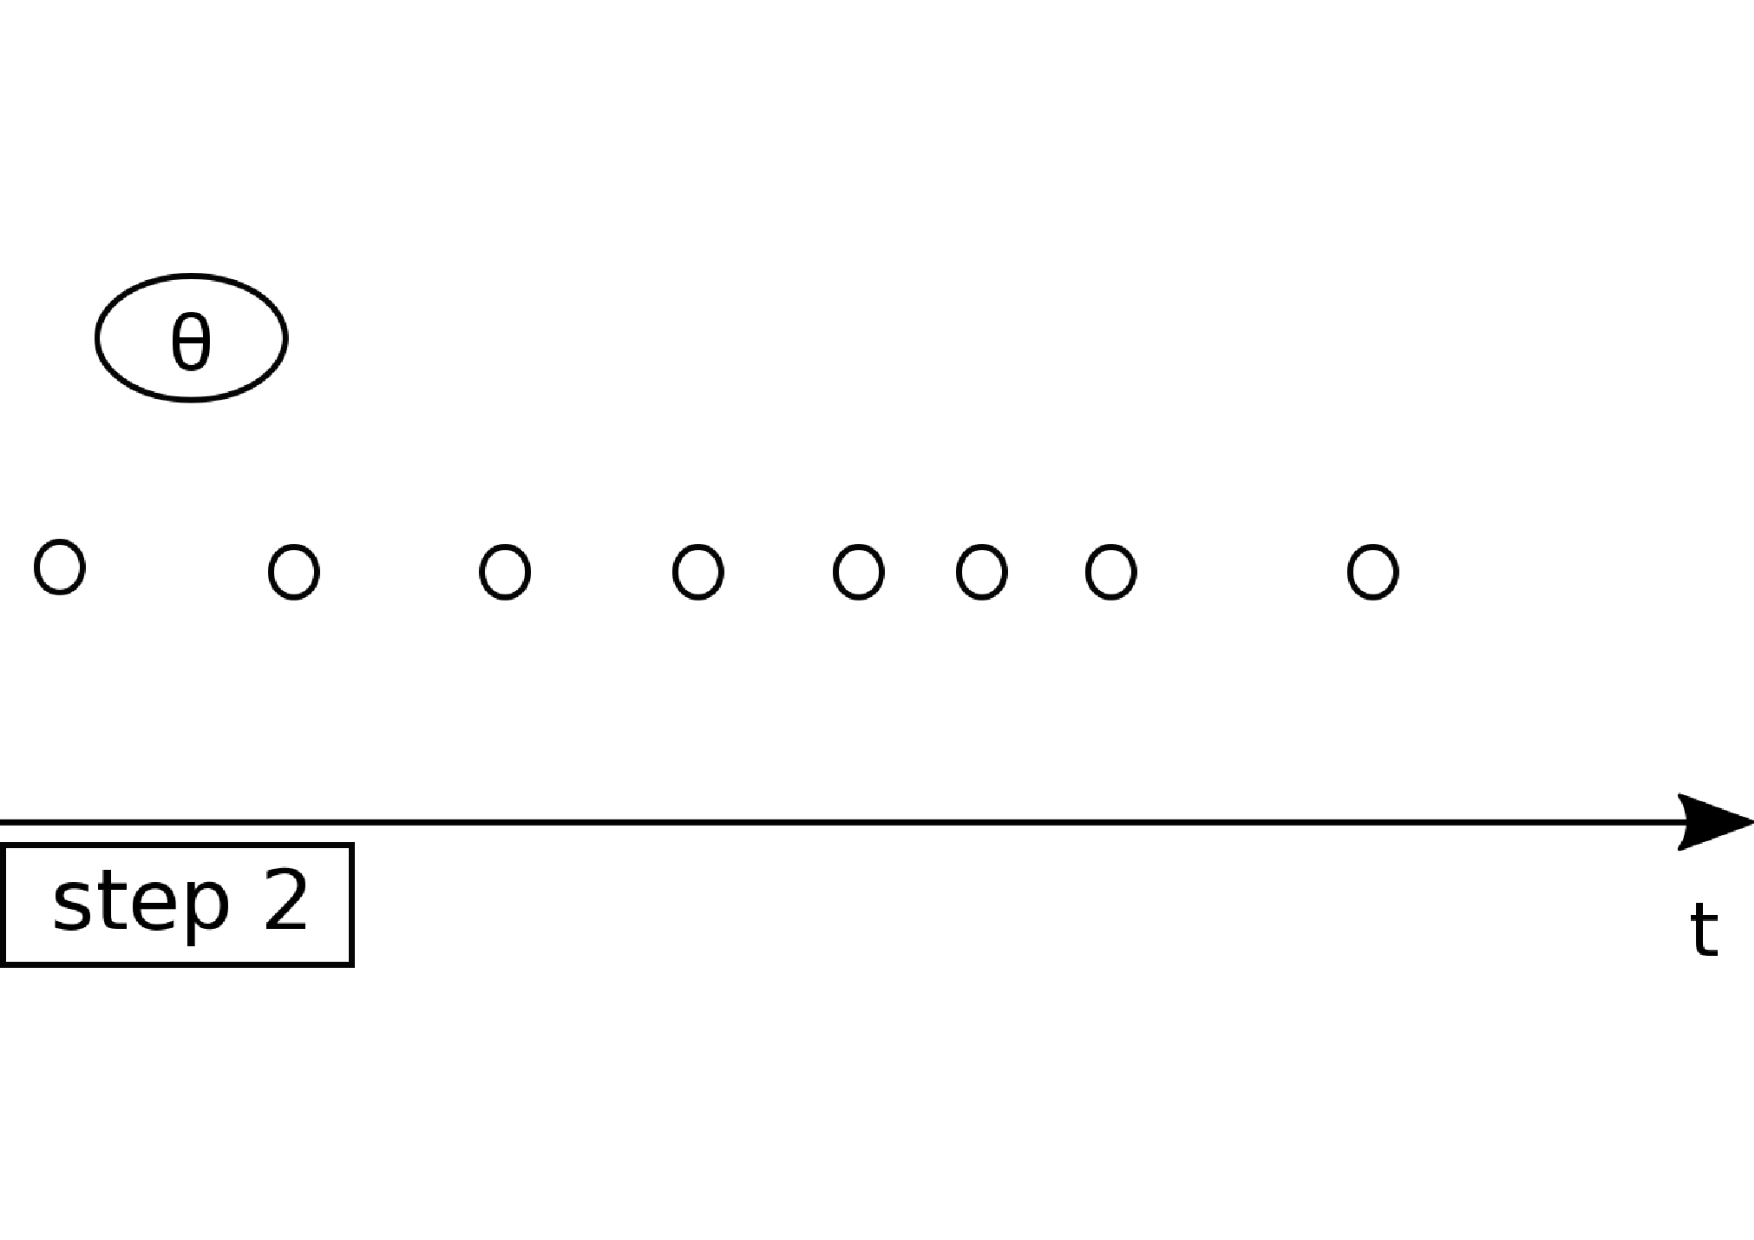
\includegraphics [width=0.70\textwidth, angle=0]{figs/plotn2.pdf}
    \vspace{-0 in}
  \end{minipage}
  \begin{minipage}[!hp]{0.45\linewidth}
  \centering
    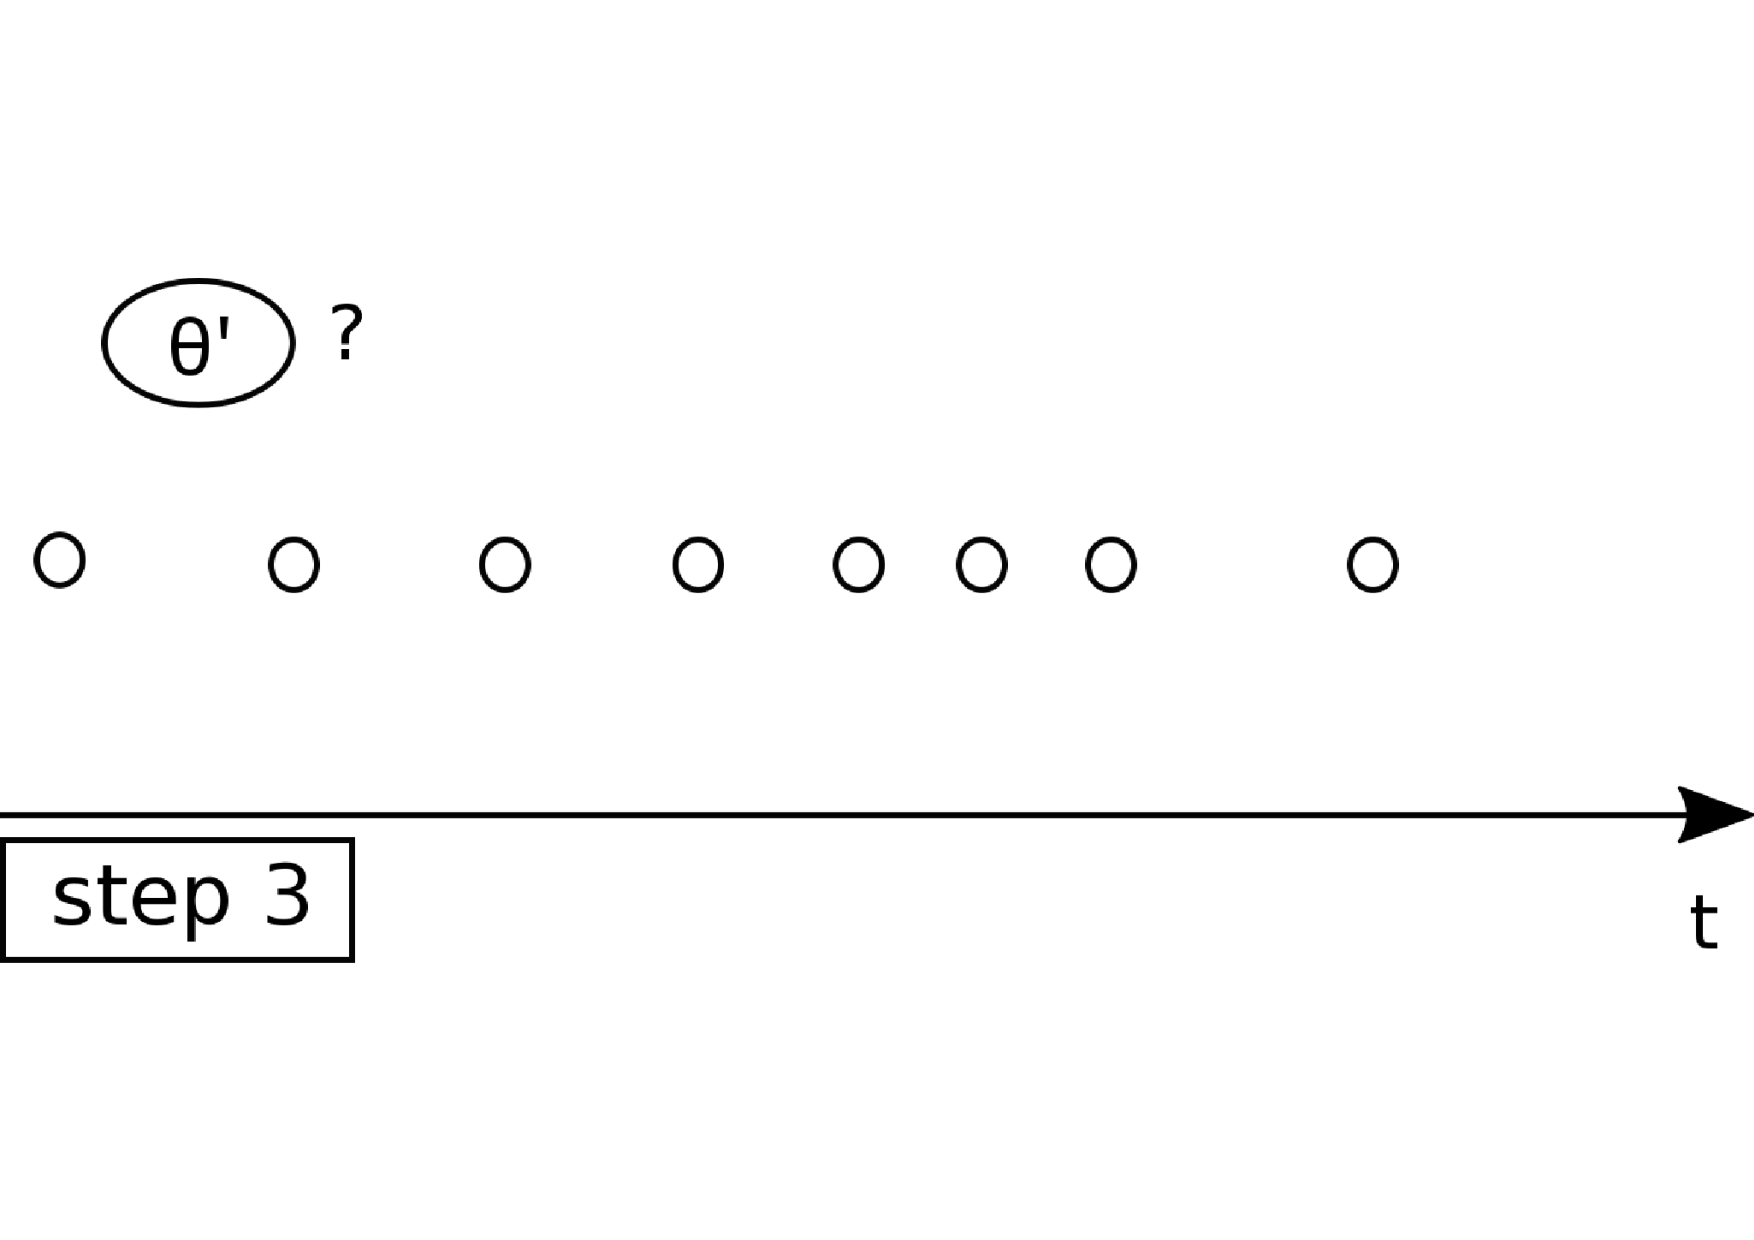
\includegraphics [width=0.70\textwidth, angle=0]{figs/plotn3.pdf}
    \vspace{-0 in}
  \end{minipage}
  \begin{minipage}[!hp]{0.45\linewidth}
  \centering
    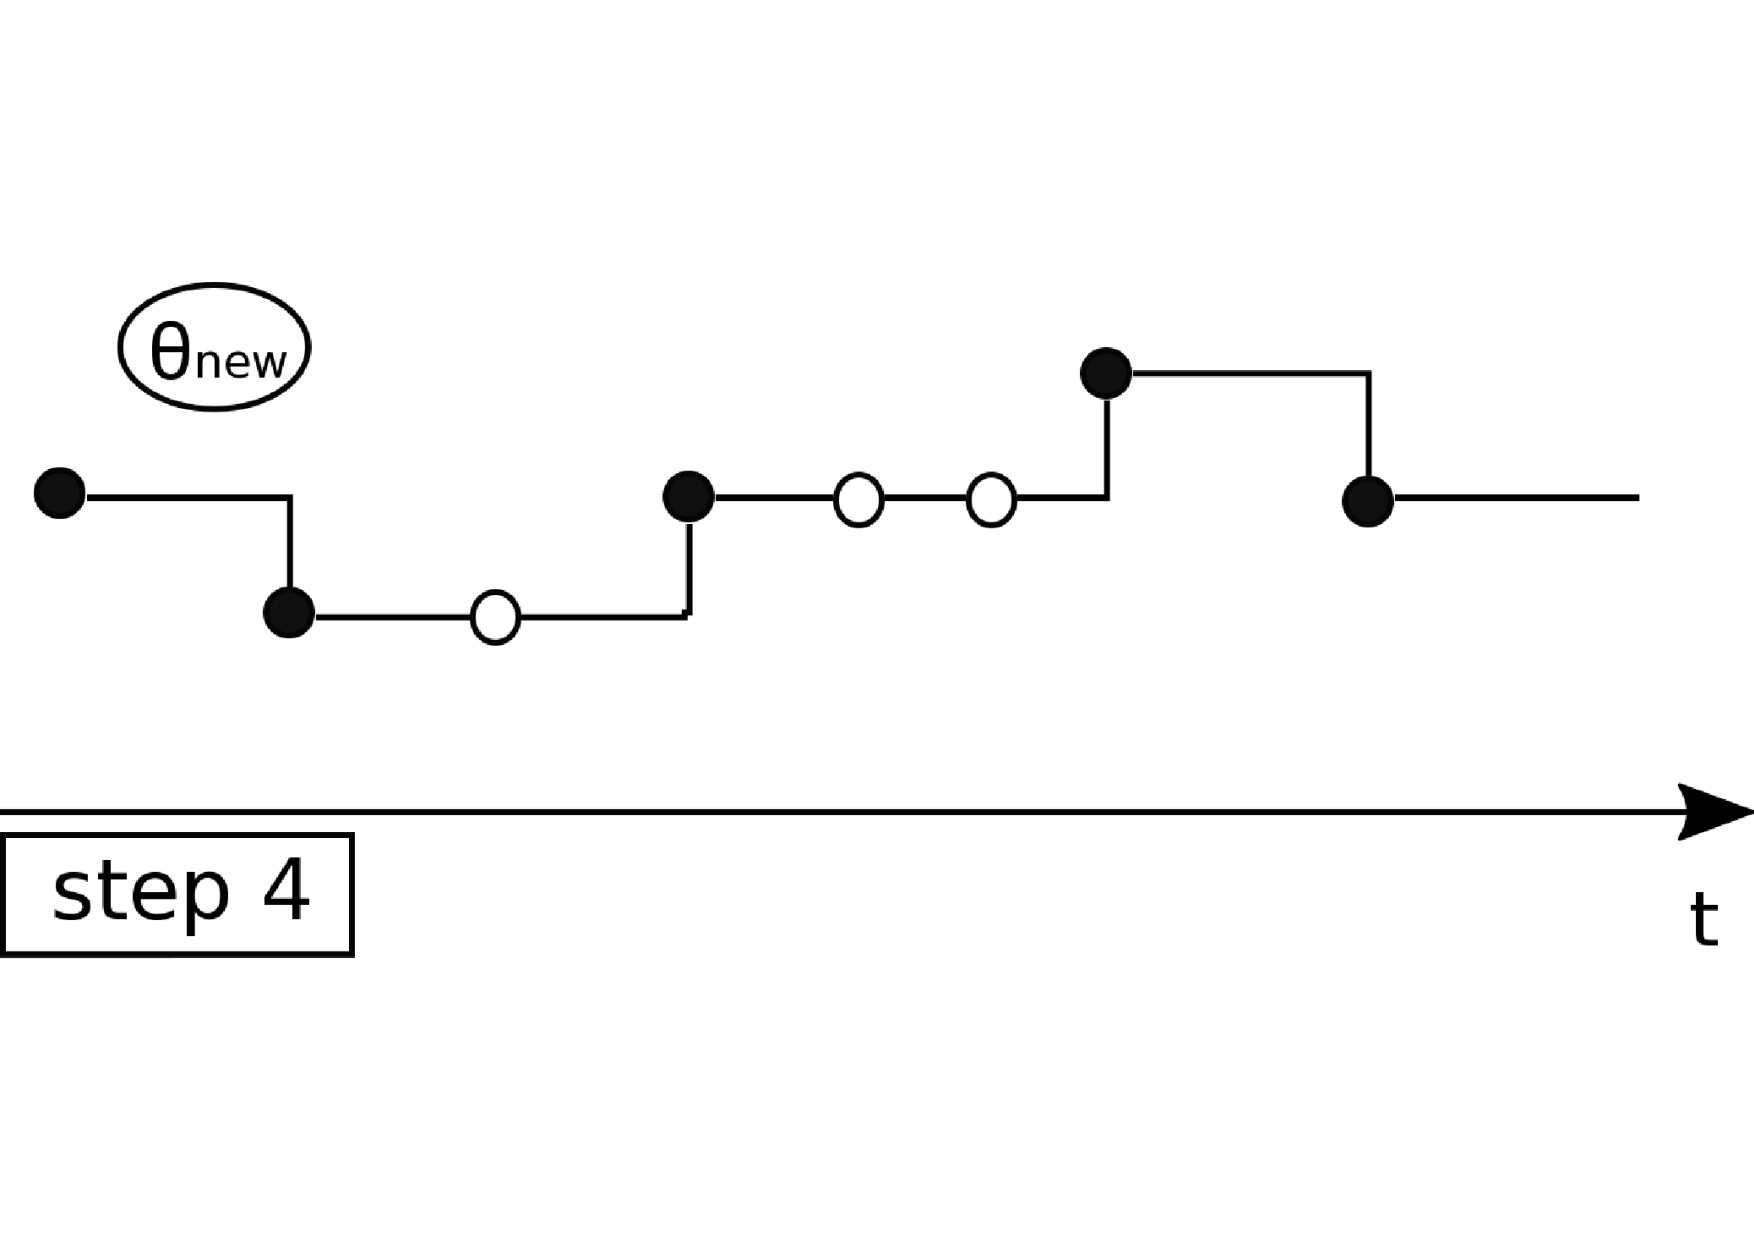
\includegraphics [width=0.70\textwidth, angle=0]{figs/plotn4.pdf}
    \vspace{-0 in}
  \end{minipage}
  \begin{minipage}[!hp]{0.45\linewidth}
  \centering
    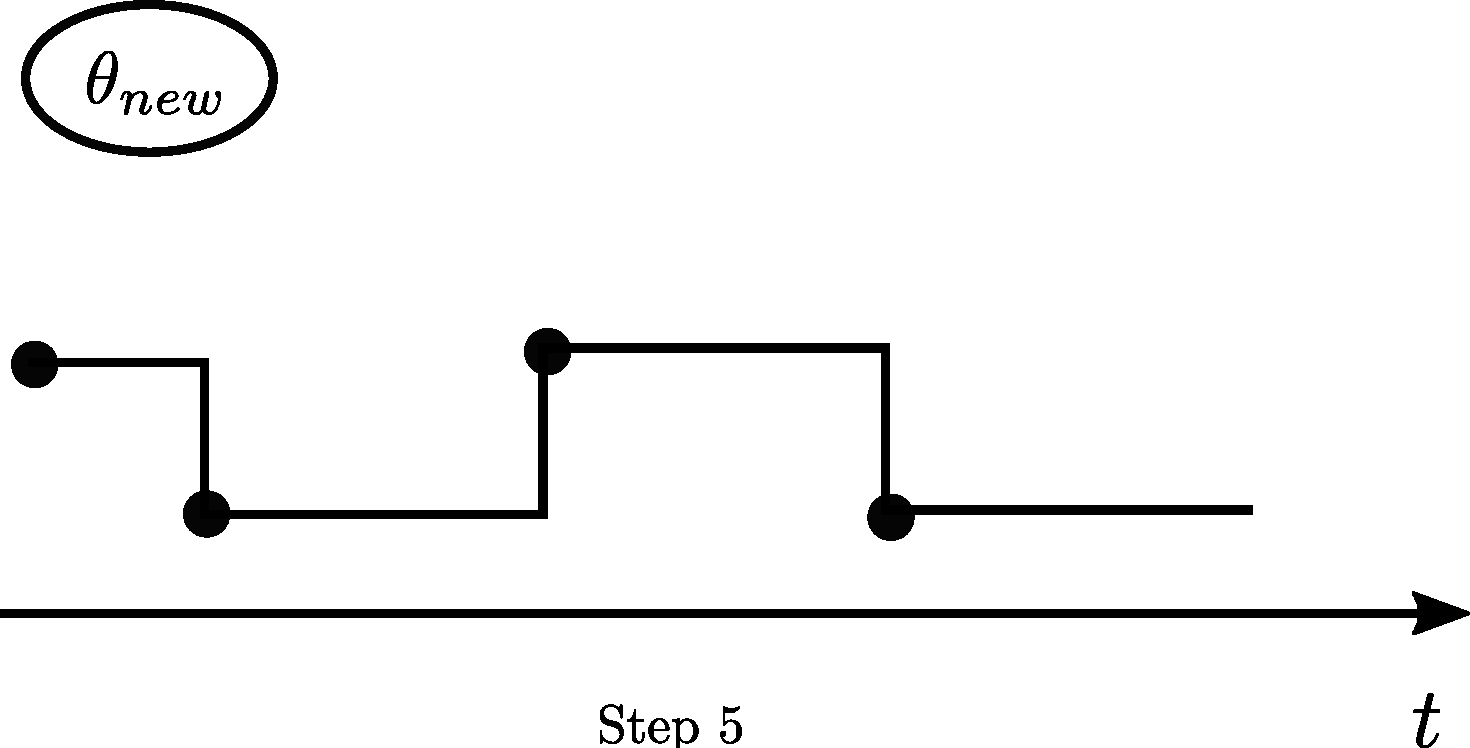
\includegraphics [width=0.70\textwidth, angle=0]{figs/plotn5.pdf}
    \vspace{-0 in}
  \end{minipage}
  \caption{\Naive\ MH-algorithm: Step 0 to 2: sample thinned events
  and discard state information to get a random grid. Step 3: 
propose a new parameter $\theta'$, and accept or reject by making
a forward pass on the grid. Steps 4 to 5: make a backward pass using
the accepted parameter and discard self-transitions to produce a new
trajectory.}
   \label{fig:naive_mh}
  \end{figure}

\subsection{Additional results}
\vspace{-.4in}
  \begin{figure}[H]
  \centering
  \begin{minipage}[h!]{0.65\linewidth}
  \centering
    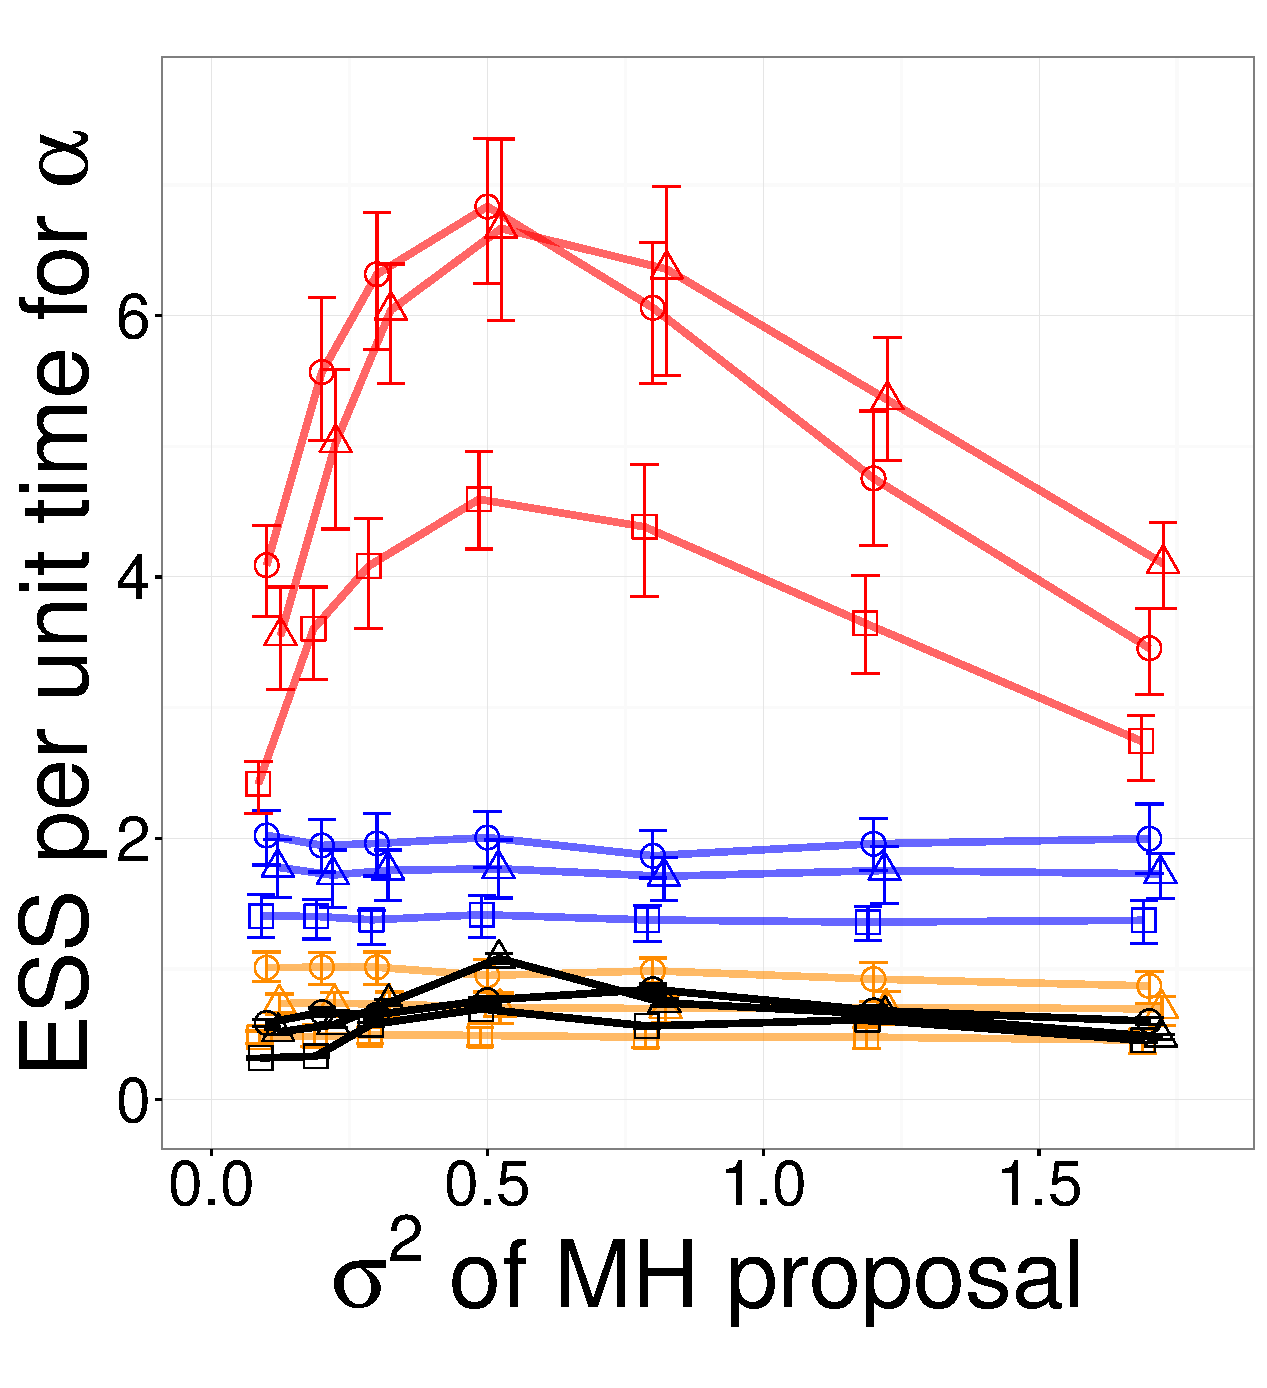
\includegraphics [width=0.44\textwidth, angle=0]{figs/exp_5_alpha.pdf}
    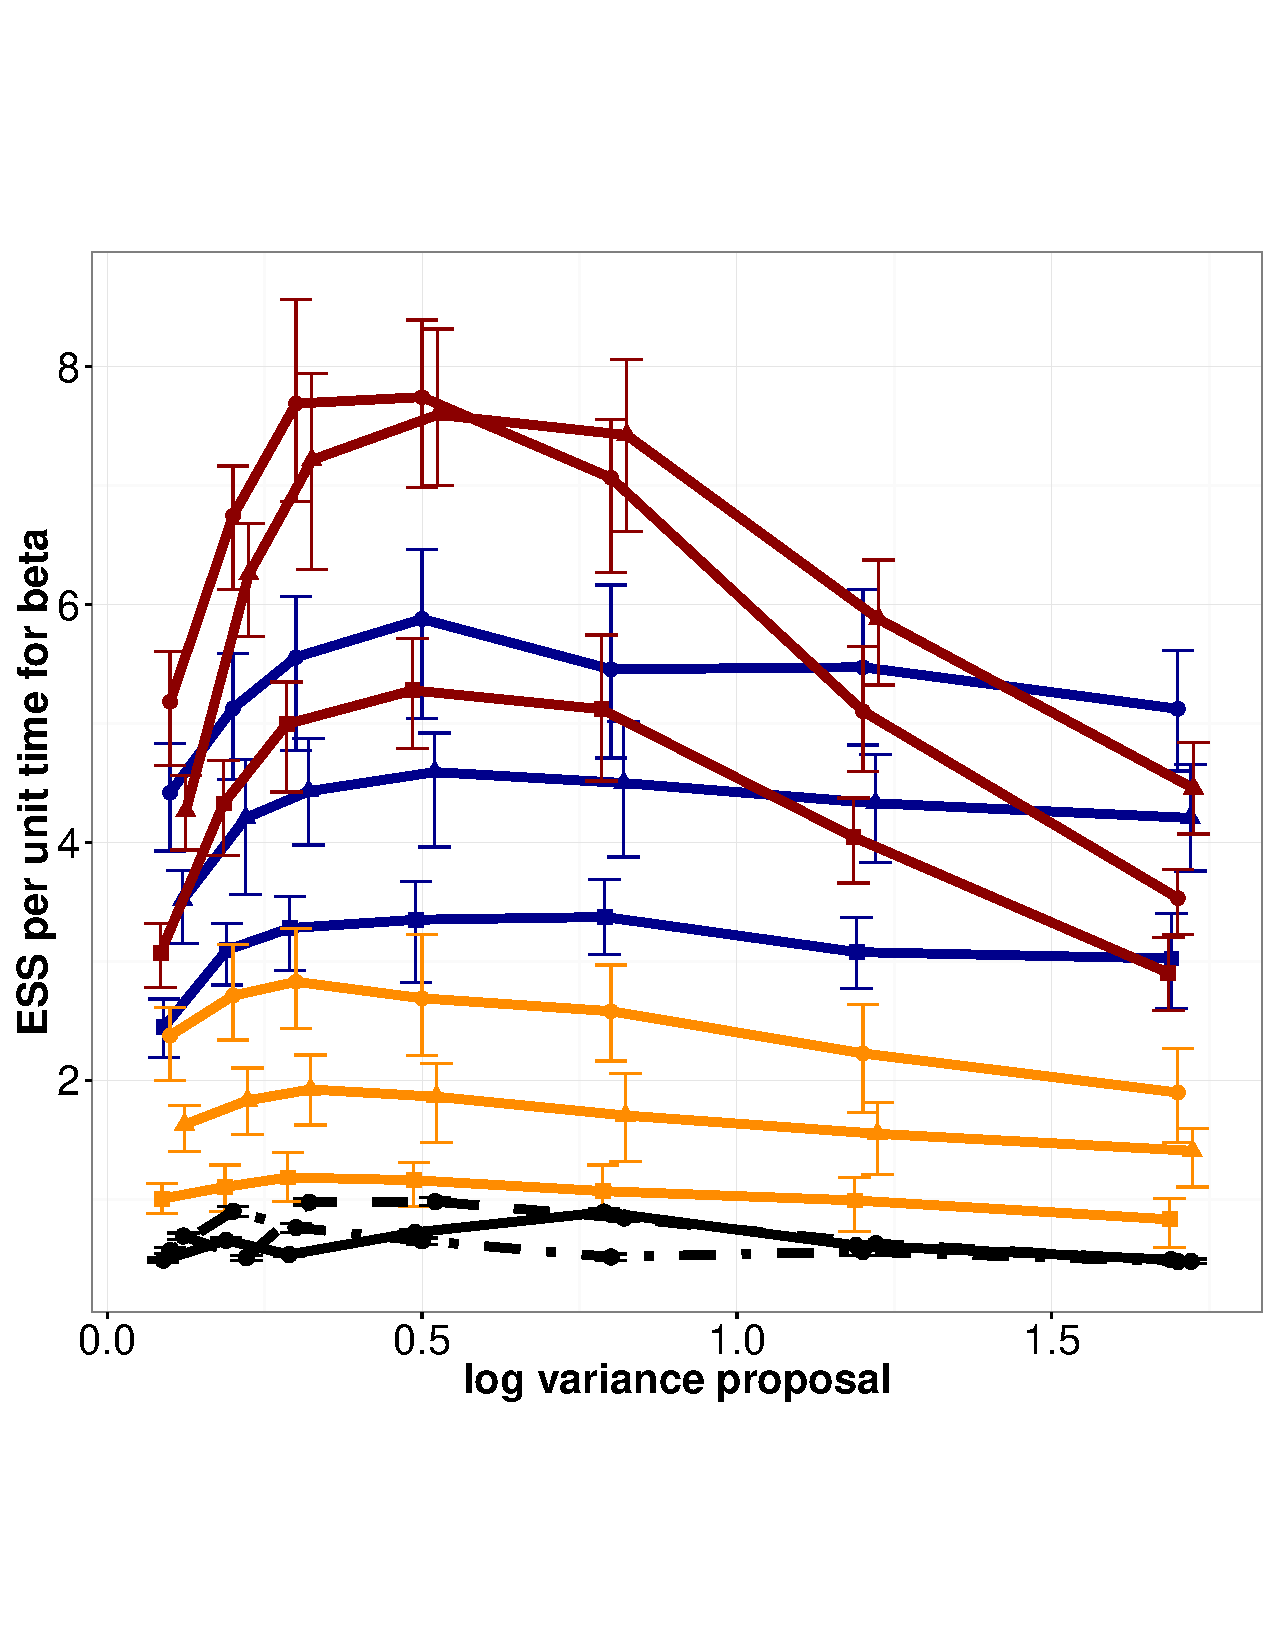
\includegraphics [width=0.44\textwidth, angle=0]{figs/exp_5_beta.pdf}
  \end{minipage}
  \begin{minipage}[!hp]{0.33\linewidth}
    \caption{ESS/sec for the synthetic  model, dimension 5. (Left, right) 
      are $(\alpha, \beta)$. Red, yellow, blue and black are the symmetrized MH,
  \naive\ MH, Gibbs and particle MCMC algorithm. Different symbols are
different settings of the algorithms, see section~\ref{sec:expts}.}
     \label{fig:ESS_EXP_D5}
  \end{minipage}
  \end{figure}
  %\centering

  \begin{figure}[H]
%    \vspace{-.2in}
  \centering

  \begin{minipage}[!hp]{0.99\linewidth}
    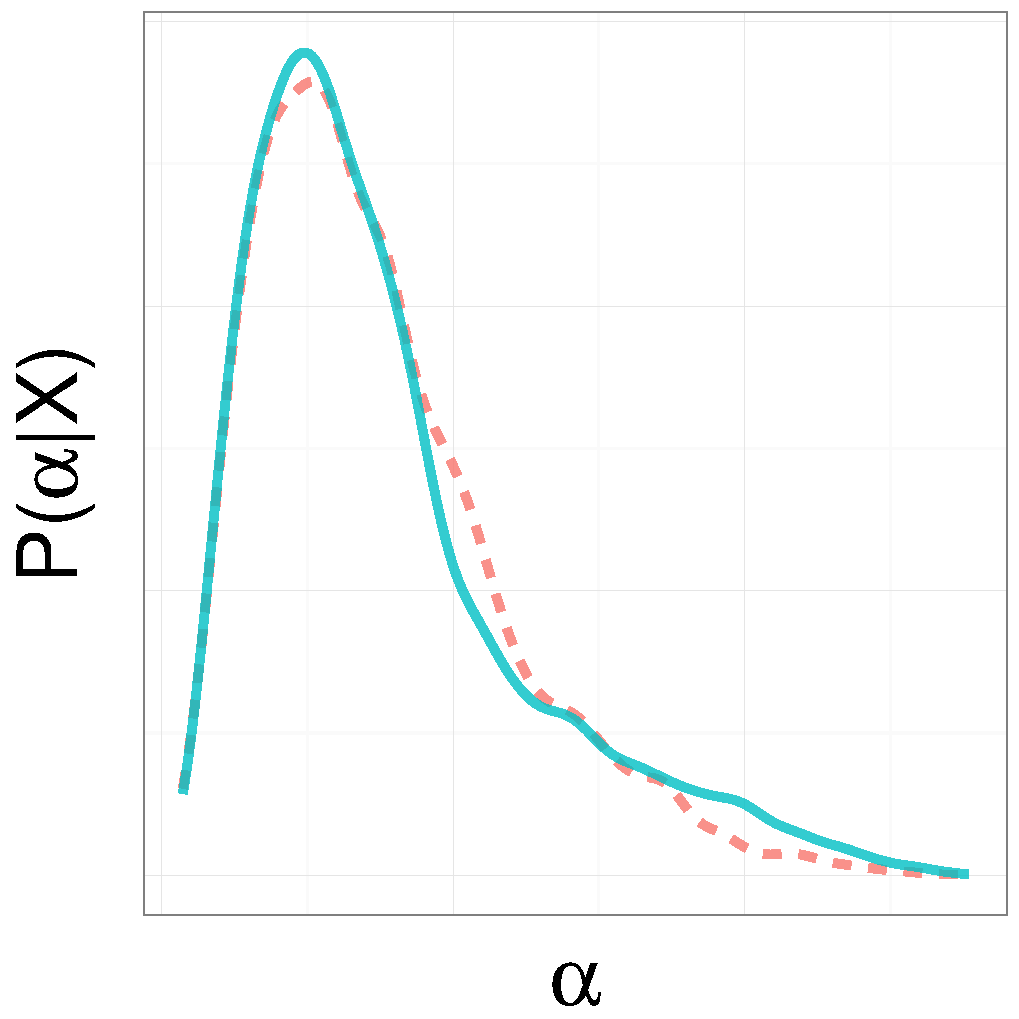
\includegraphics [width=0.3\textwidth, angle=0]{figs/EXP_ks/exp_hist_44_05_10_.pdf}
    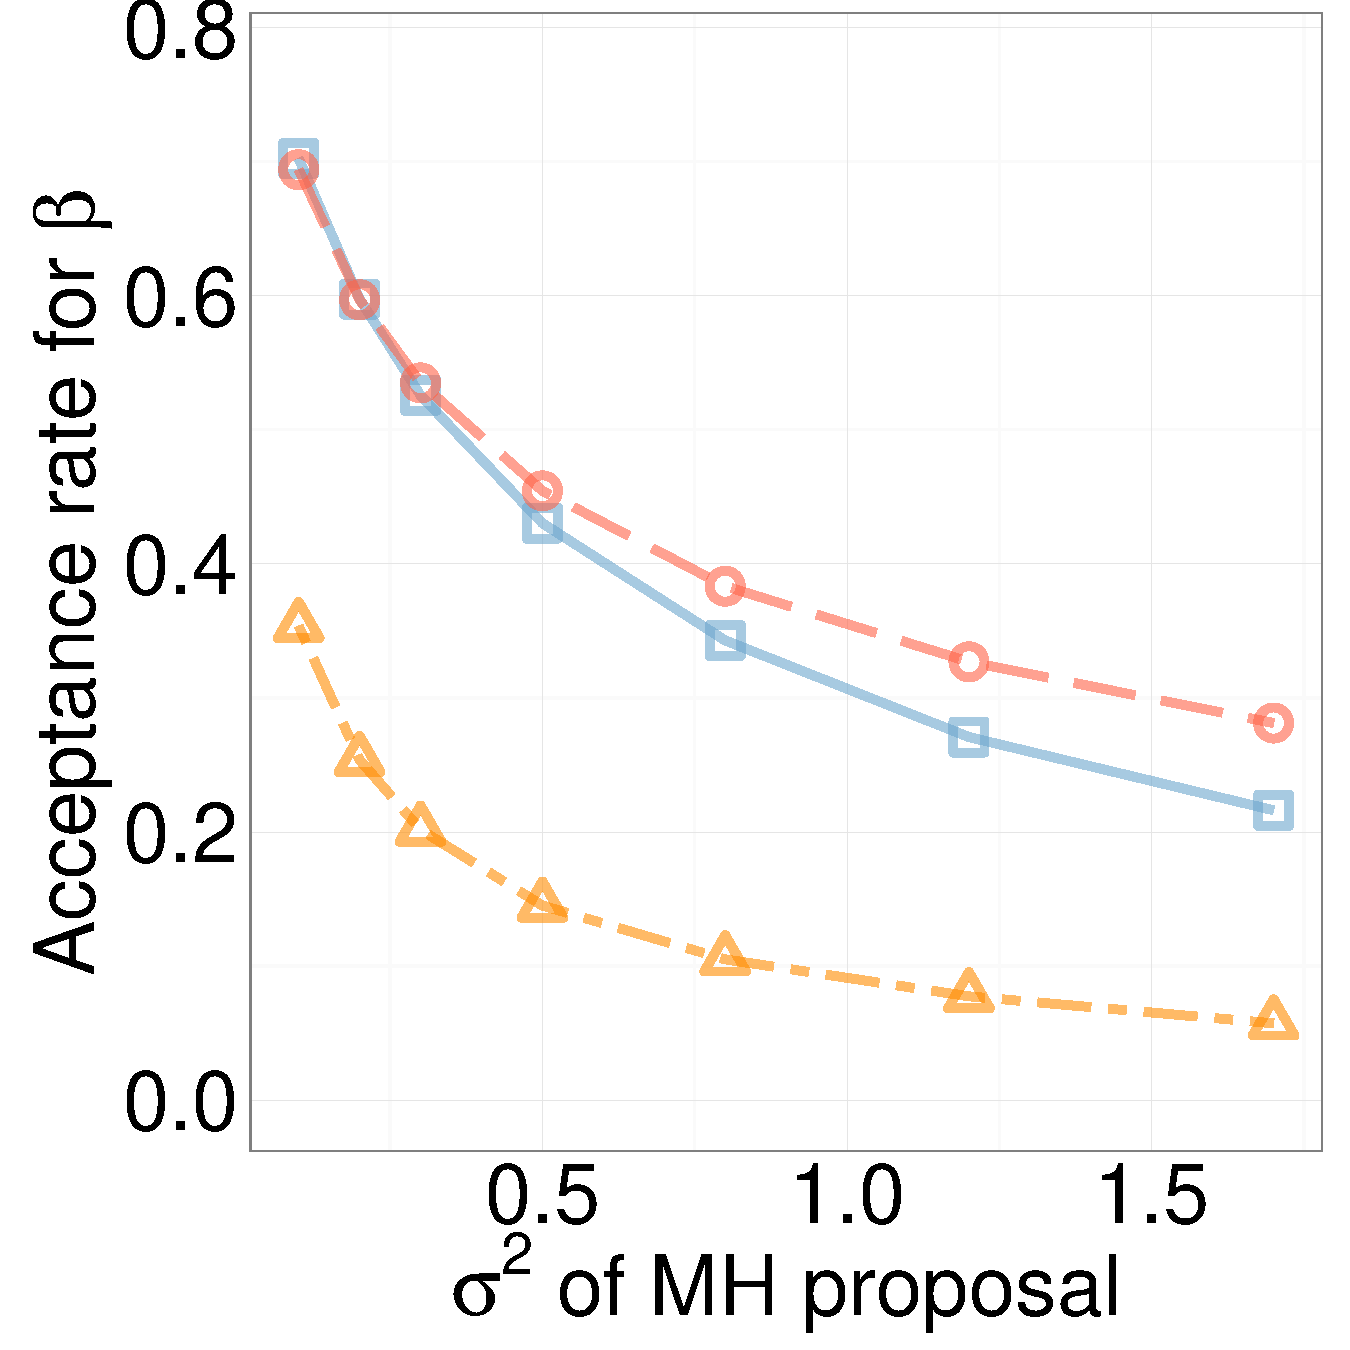
\includegraphics [width=0.30\textwidth, angle=0]{figs/acc/EXP_D3beta_k2.pdf}
	\hspace{.5in}
    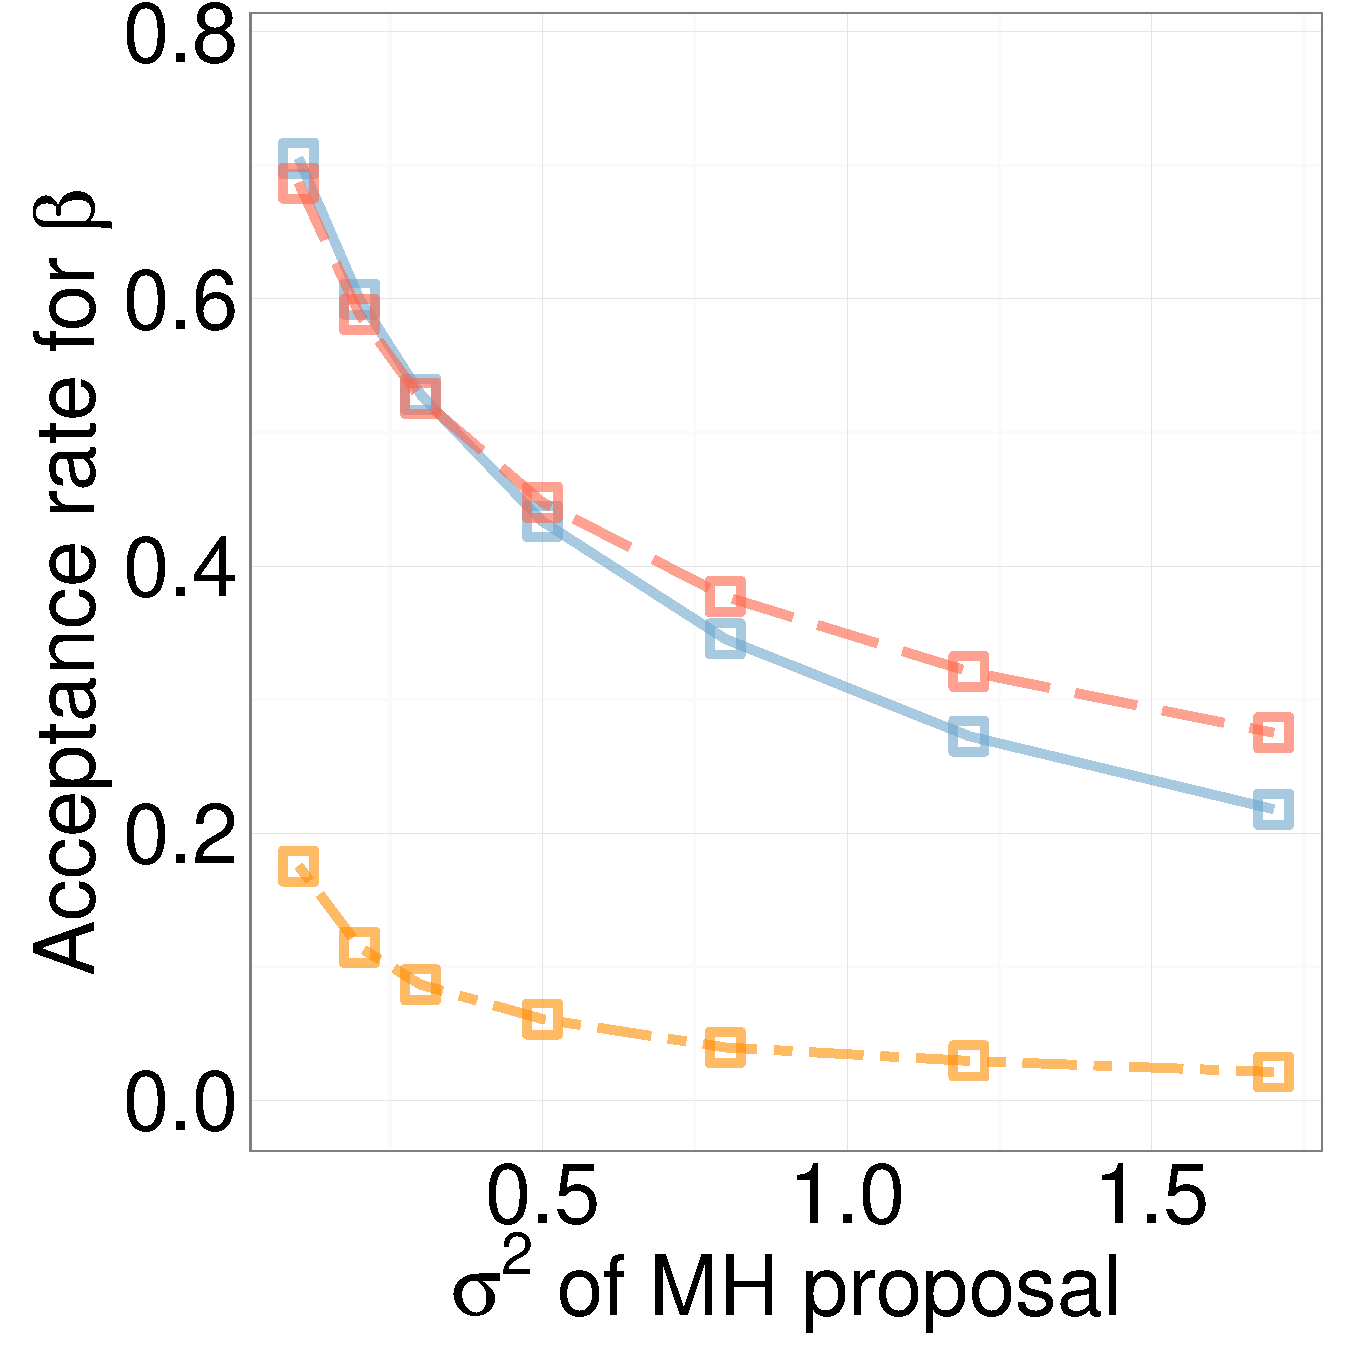
\includegraphics [width=0.30\textwidth, angle=0]{figs/acc/EXP_D10beta_k2.pdf}
  \end{minipage}
%  \begin{minipage}[!hp]{0.99\linewidth}
    \caption{Acceptance Rate for $\beta$ in the synthetic model, the left row being dimension 3, and the right,dimension 10.  Red, yellow and blue curves are the Gibbs, symmetrized MH,
 and \naive\ MH  algorithm. The multiplicative factor is $2$. }
     \label{fig:ACC_EXP}
%  \end{minipage}
  \end{figure}
  \begin{figure}[H]
%    \vspace{-.2in}
  \centering

  \begin{minipage}[!hp]{0.99\linewidth}
  	\centering
    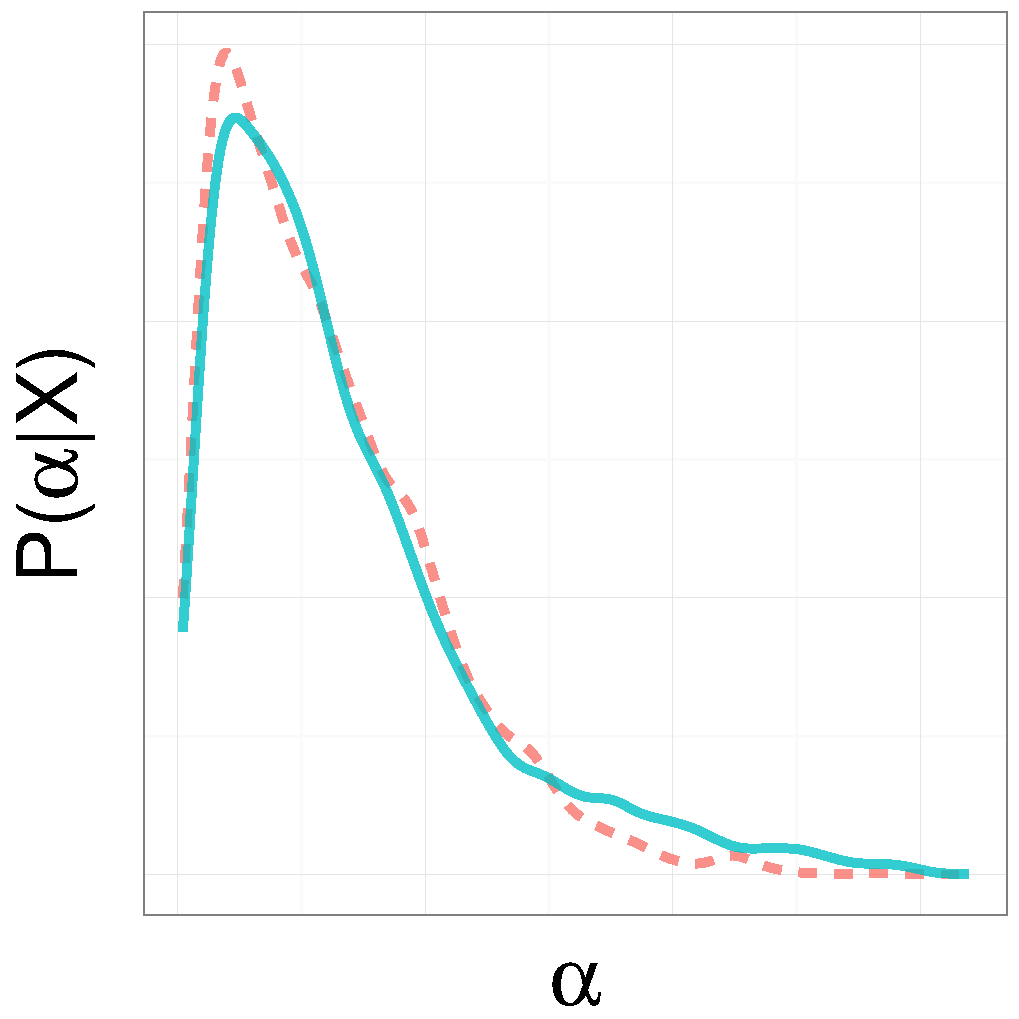
\includegraphics [width=0.3\textwidth, angle=0]{figs/JC_ks/jc_hist_44_05_3_.pdf}
    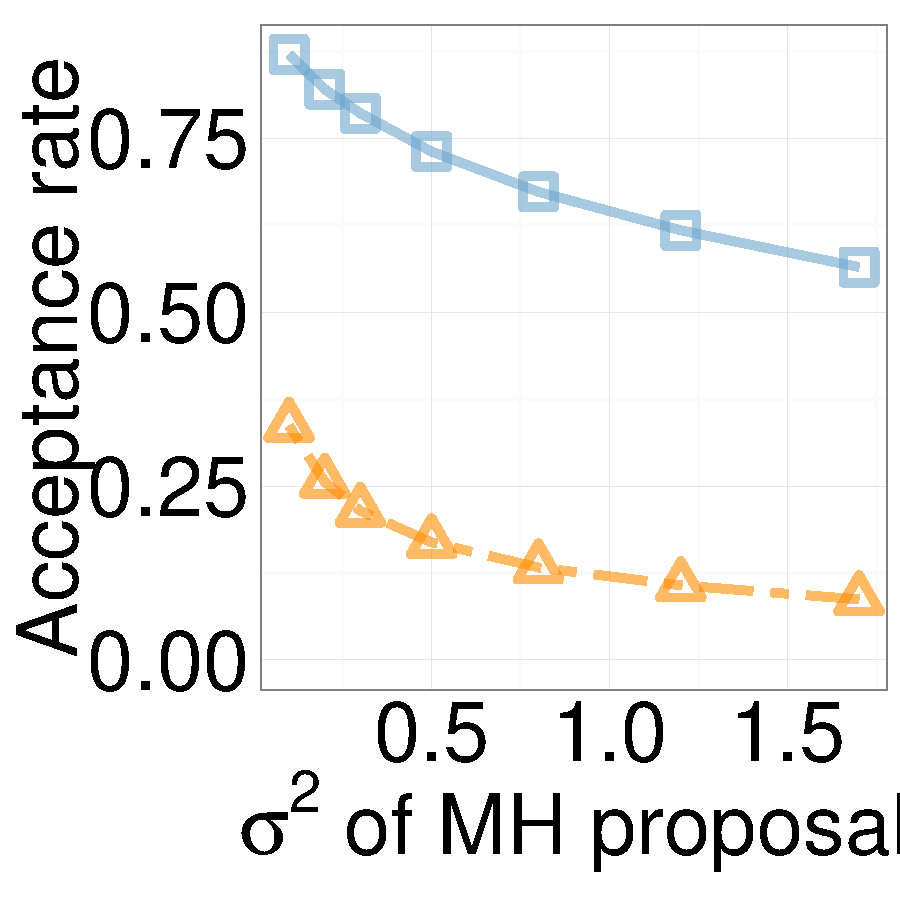
\includegraphics [width=0.3\textwidth, angle=0]{figs/acc/JCalpha_k2.pdf}
	\hspace{.5in}
    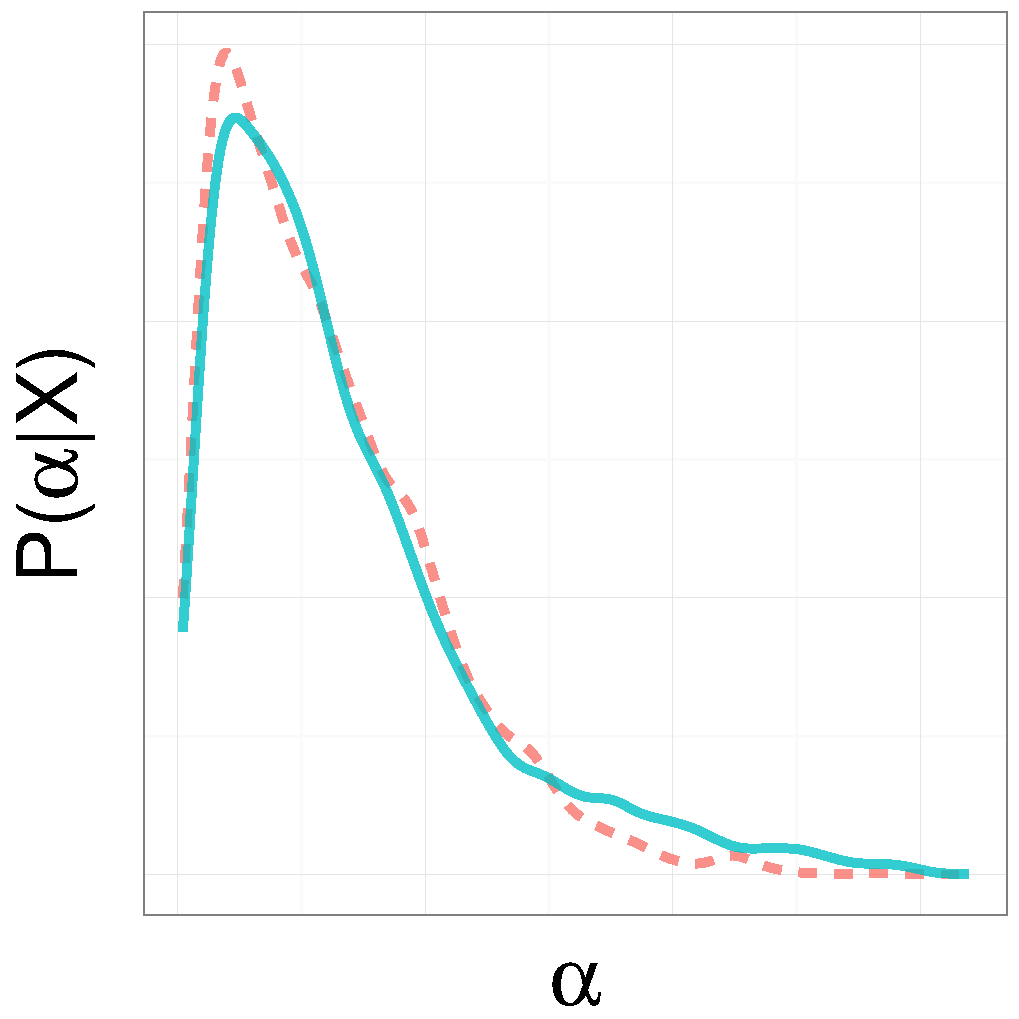
\includegraphics [width=0.3\textwidth, angle=0]{figs/JC_ks/jc_hist_44_05_3_.pdf}
  \end{minipage}
%  \begin{minipage}[!hp]{0.99\linewidth}
    \caption{The left represents the acceptance rate for $\alpha$ in the JC69 model.  Yellow and blue curves represent symmetrized MH,and \naive\ MH  algorithm. The multiplicative factor is $2$.The right is histogram for the posterior samples($\alpha$ ) of the JC69 model, the red and blue curves are the Gibbs and symmetrized MH. The p value of the two sample-Kolmogorov Smirnov test is $ 0.97$.  }
     \label{fig:ACC_JC}
%  \end{minipage}
  \end{figure}
  
  \begin{figure}[H]
%    \vspace{-.2in}
  \centering
%  \begin{minipage}[!hp]{0.99\linewidth}
 % \centering
  \begin{minipage}[!hp]{0.99\linewidth}
    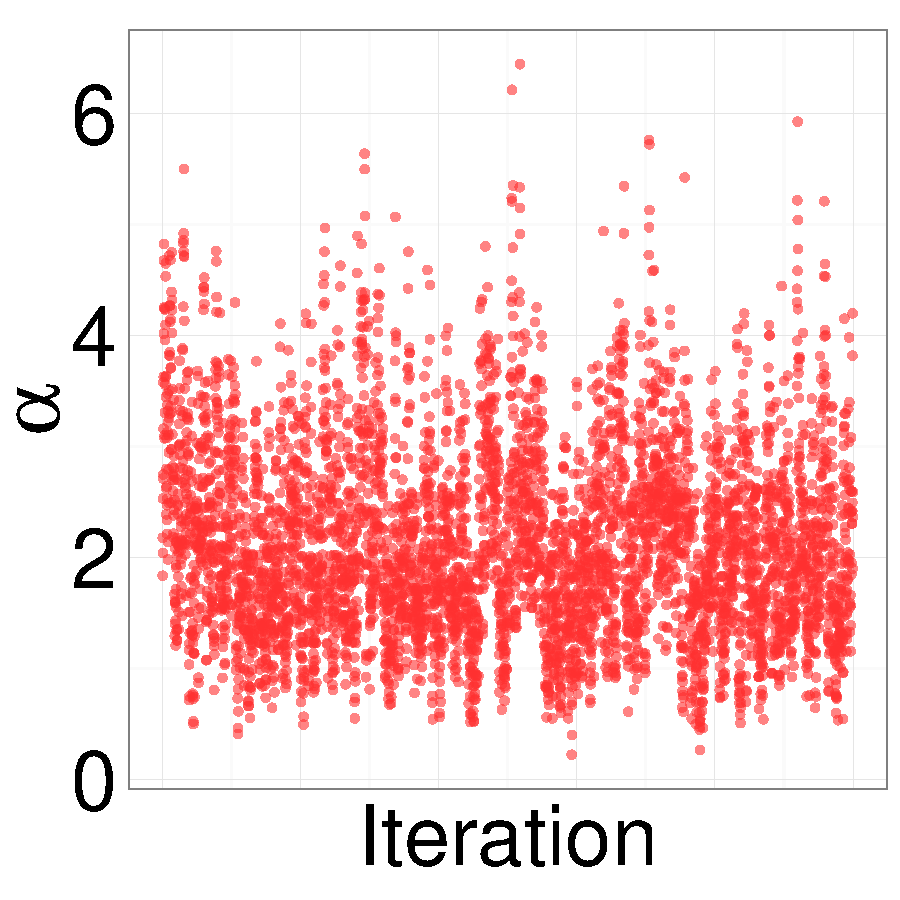
\includegraphics [width=0.24\textwidth, angle=0]{figs/Q_ks/q_traceGBS_20_03_3_.pdf}
    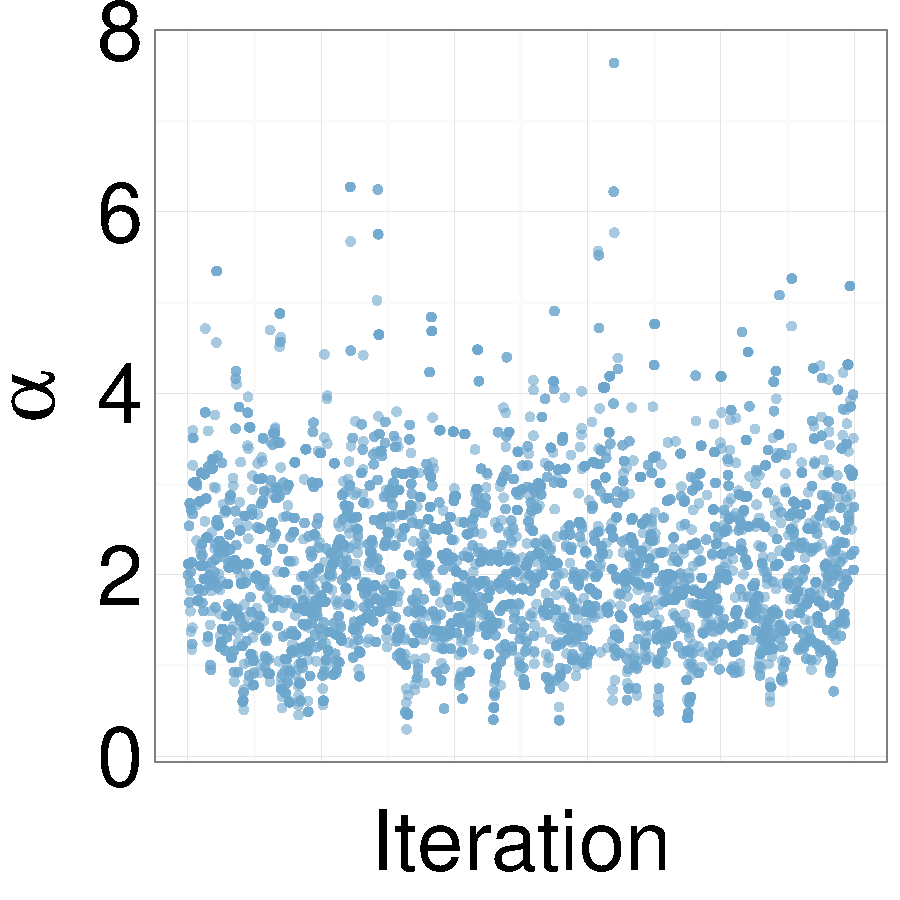
\includegraphics [width=0.24\textwidth, angle=0]{figs/Q_ks/q_traceMH_20_03_3_.pdf}
    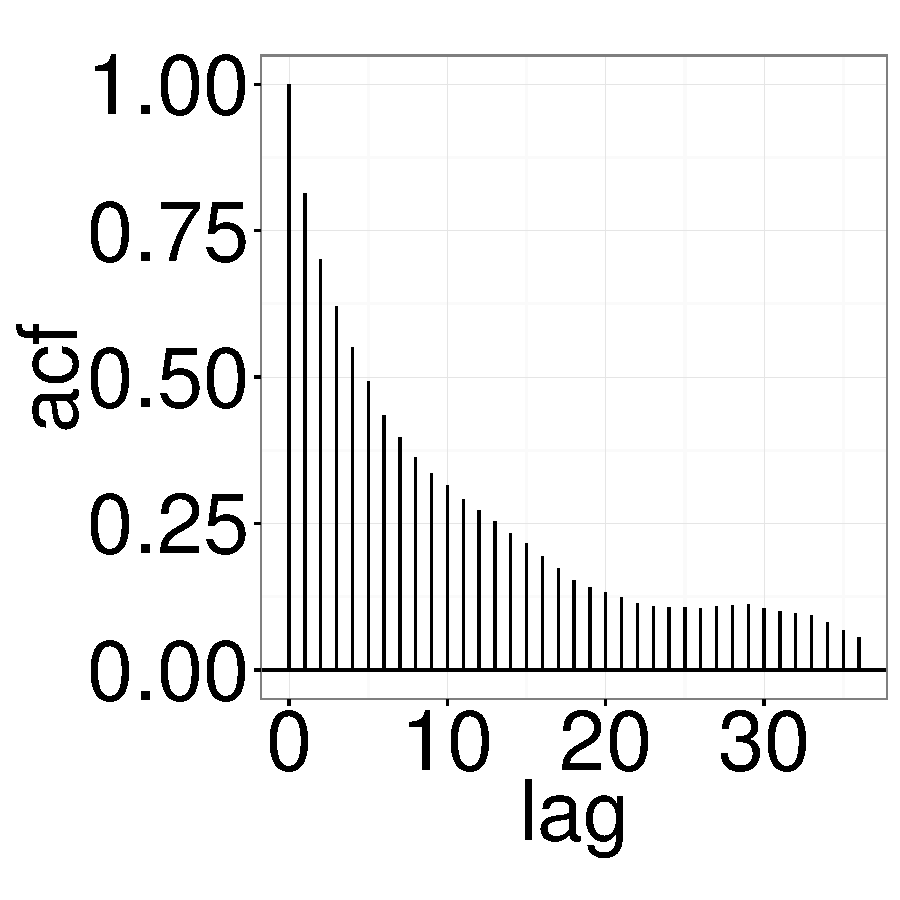
\includegraphics [width=0.24\textwidth, angle=0]{figs/Q_ks/q_gbsacf_20_03_3_.pdf}
    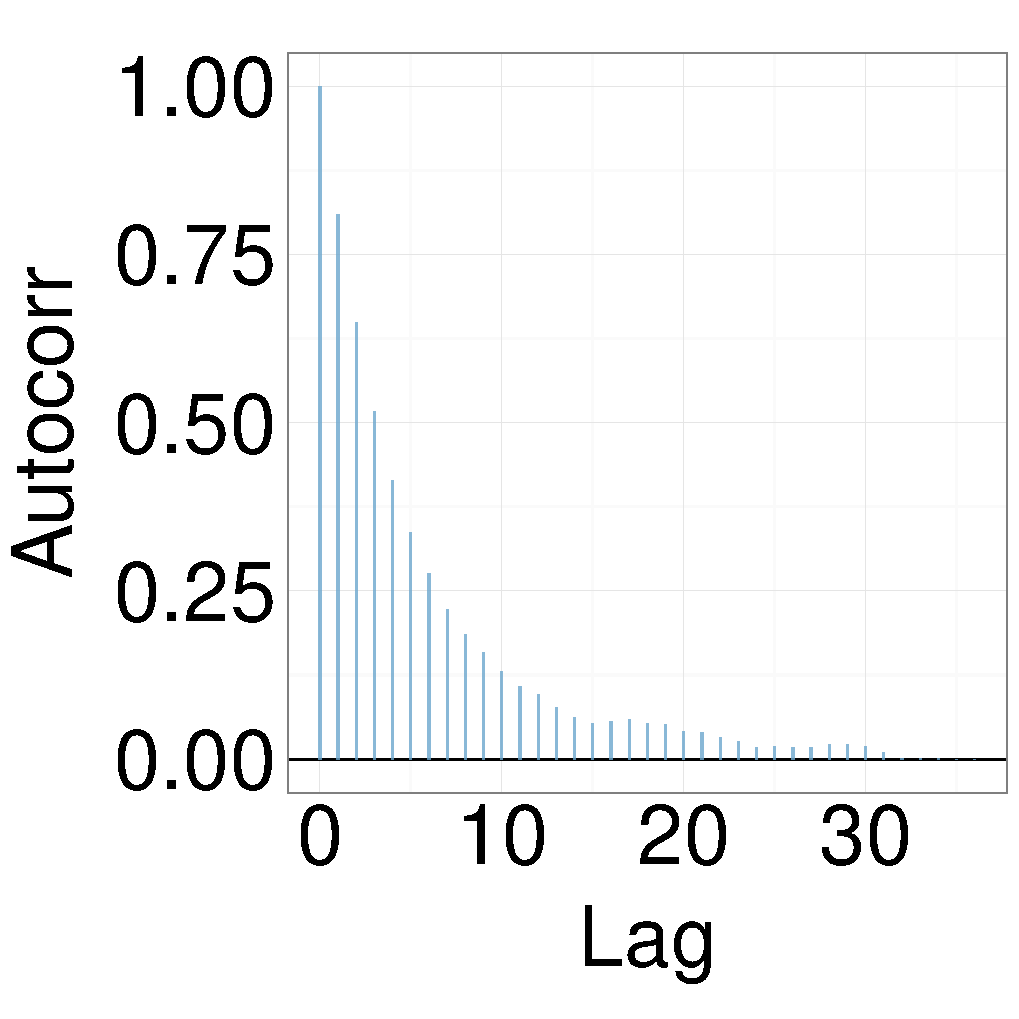
\includegraphics [width=0.24\textwidth, angle=0]{figs/Q_ks/q_mhacf_20_03_3_.pdf}
  \end{minipage}

%  \end{minipage}
%  \begin{minipage}[!hp]{0.99\linewidth}
    \caption{The left is histogram for the posterior samples($\alpha$) of the immigration model with dimension 3, the red and blue curves are the Gibbs and symmetrized MH. The p value of the two sample-Kolmogorov Smirnov test is $ 0.978$. The middle and the right are trace plots for the posterior samples of the immigration model with dimension 3, the middle is for Gibbs and the right is for symmetrized MH}
     \label{fig:TRACE_Q}
%  \end{minipage}
  \end{figure}
  
  \begin{figure}[H]
%    \vspace{-.2in}
  \centering
%  \begin{minipage}[!hp]{0.99\linewidth}
 % \centering
  \begin{minipage}[!hp]{0.99\linewidth}
    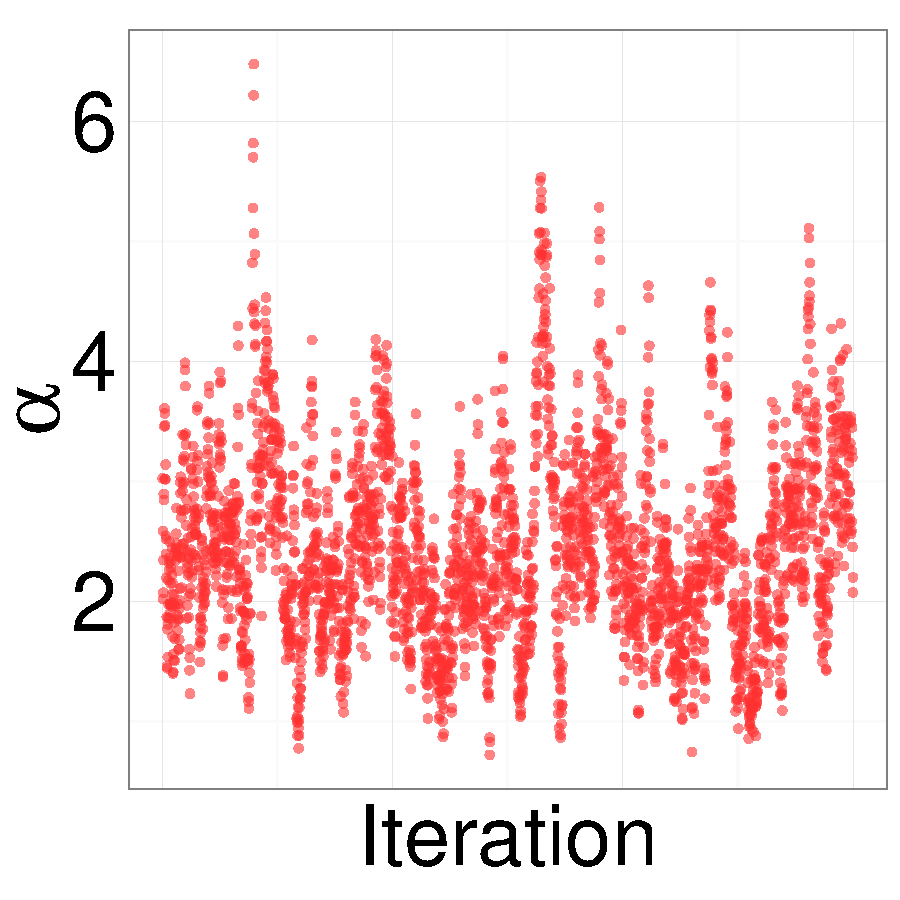
\includegraphics [width=0.24\textwidth, angle=0]{figs/QC_ks/qc_traceGBS_4_03_10_.pdf}
    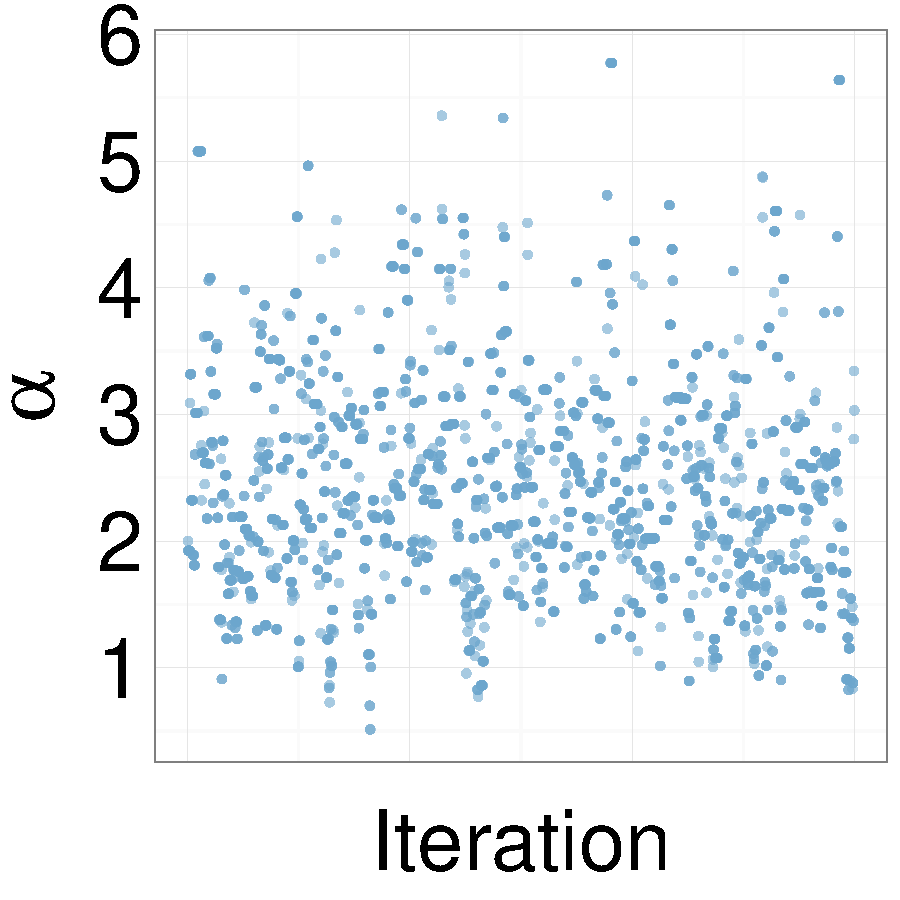
\includegraphics [width=0.24\textwidth, angle=0]{figs/QC_ks/qc_traceMH_4_03_10_.pdf}
    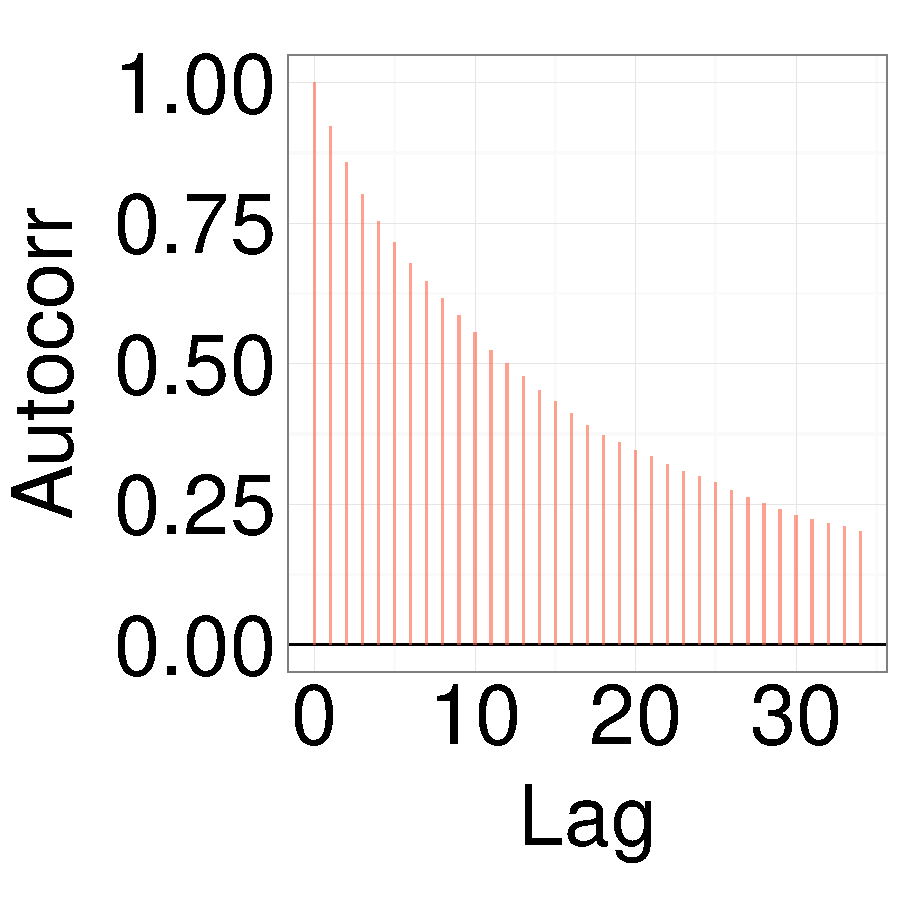
\includegraphics [width=0.24\textwidth, angle=0]{figs/QC_ks/qc_gbsacf_4_03_10_.pdf}
    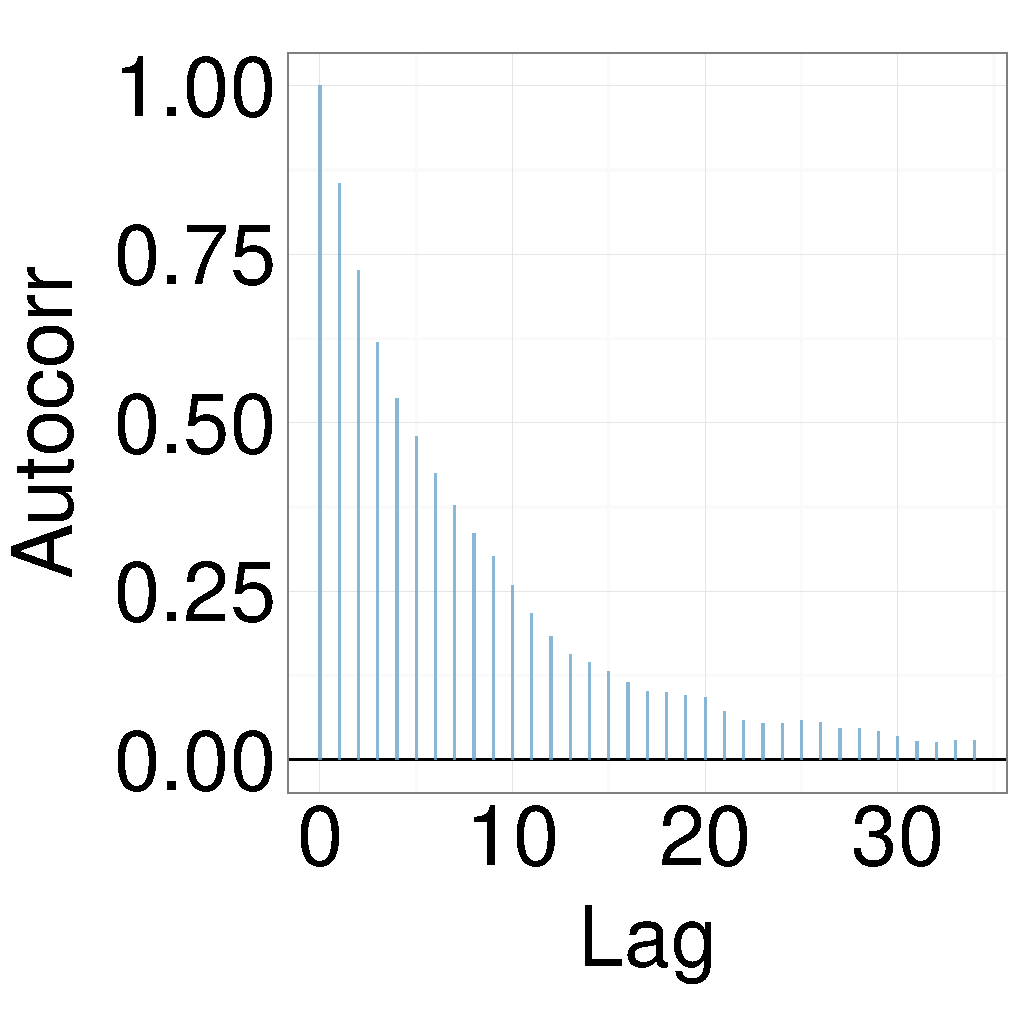
\includegraphics [width=0.24\textwidth, angle=0]{figs/QC_ks/qc_mhacf_4_03_10_.pdf}
  \end{minipage}

%  \end{minipage}
%  \begin{minipage}[!hp]{0.99\linewidth}
    \caption{The left is histogram for the posterior samples($\alpha$) of the time-inhomogeneous immigration model with dimension 10, the red and blue curves are the Gibbs and symmetrized MH. The p value of the two sample-Kolmogorov Smirnov test is $ 0.7212$. The middle and the right are trace plots for the posterior samples of the time-inhomogeneous immigration model with dimension 10, the middle is for Gibbs and the right is for symmetrized MH}
     \label{fig:TRACE_CQ}
%  \end{minipage}
  \end{figure}


  \begin{figure}[H]
  \begin{minipage}[hp]{0.65\linewidth}
  \centering
    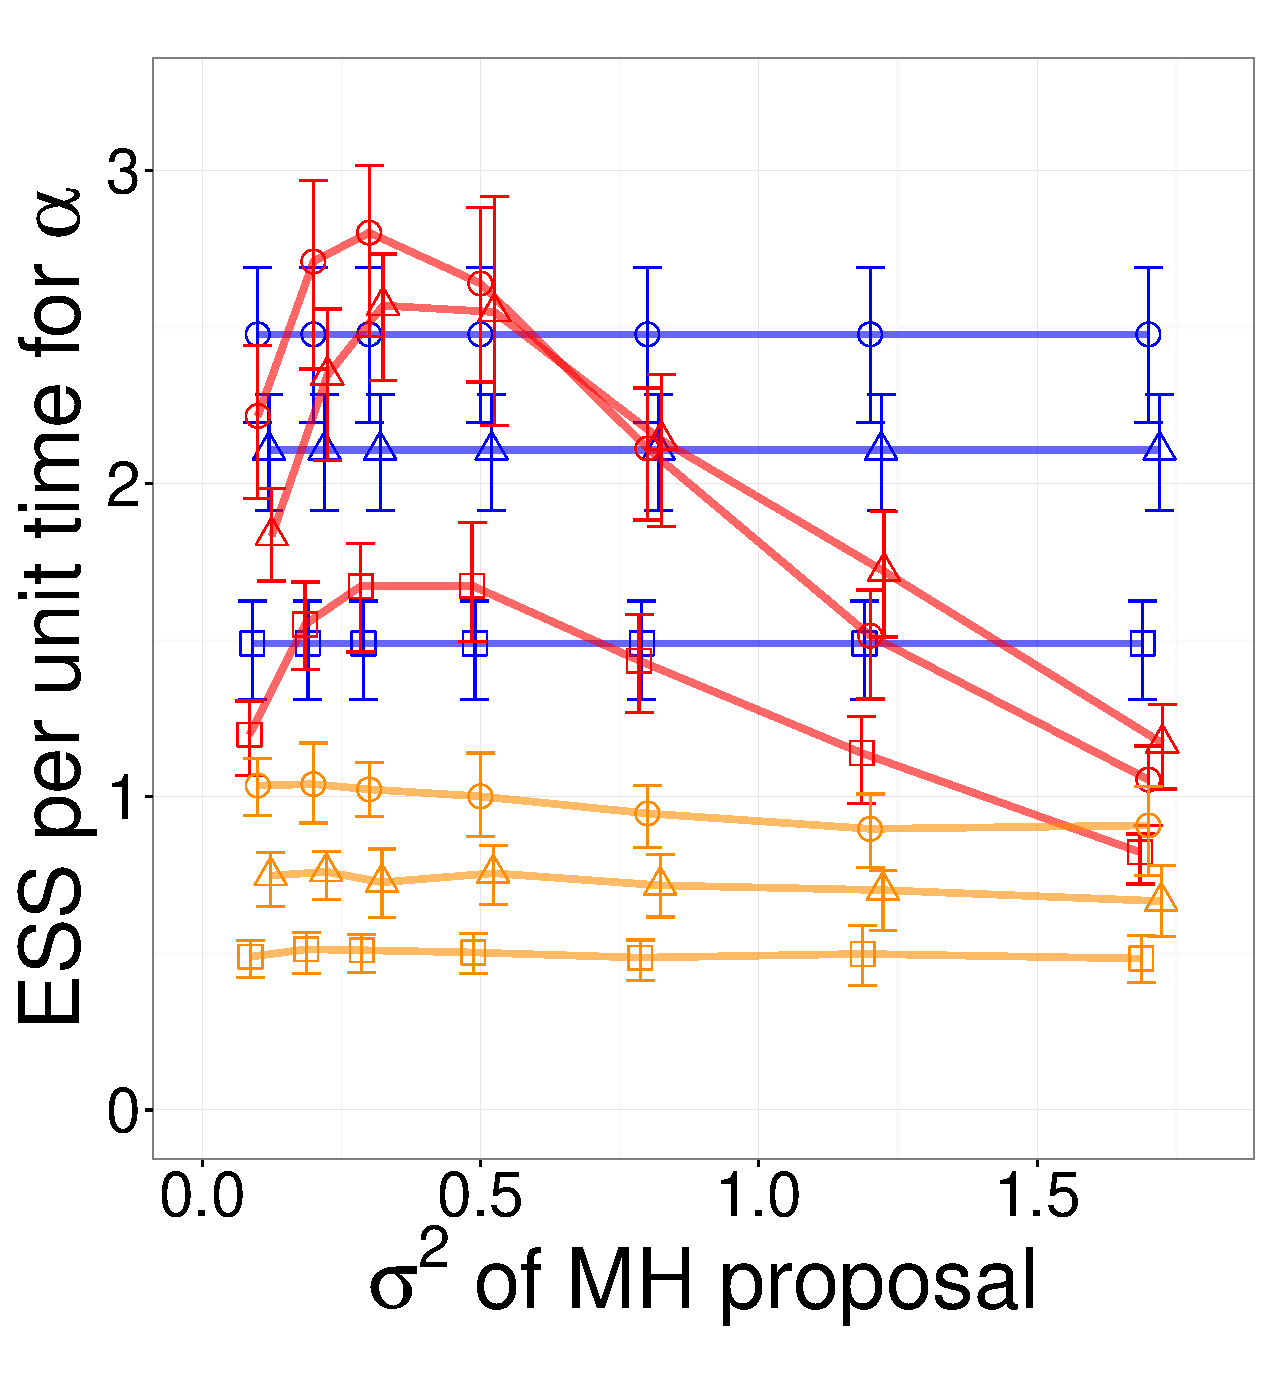
\includegraphics [width=0.44\textwidth, angle=0]{figs/q_5_alpha.pdf}
    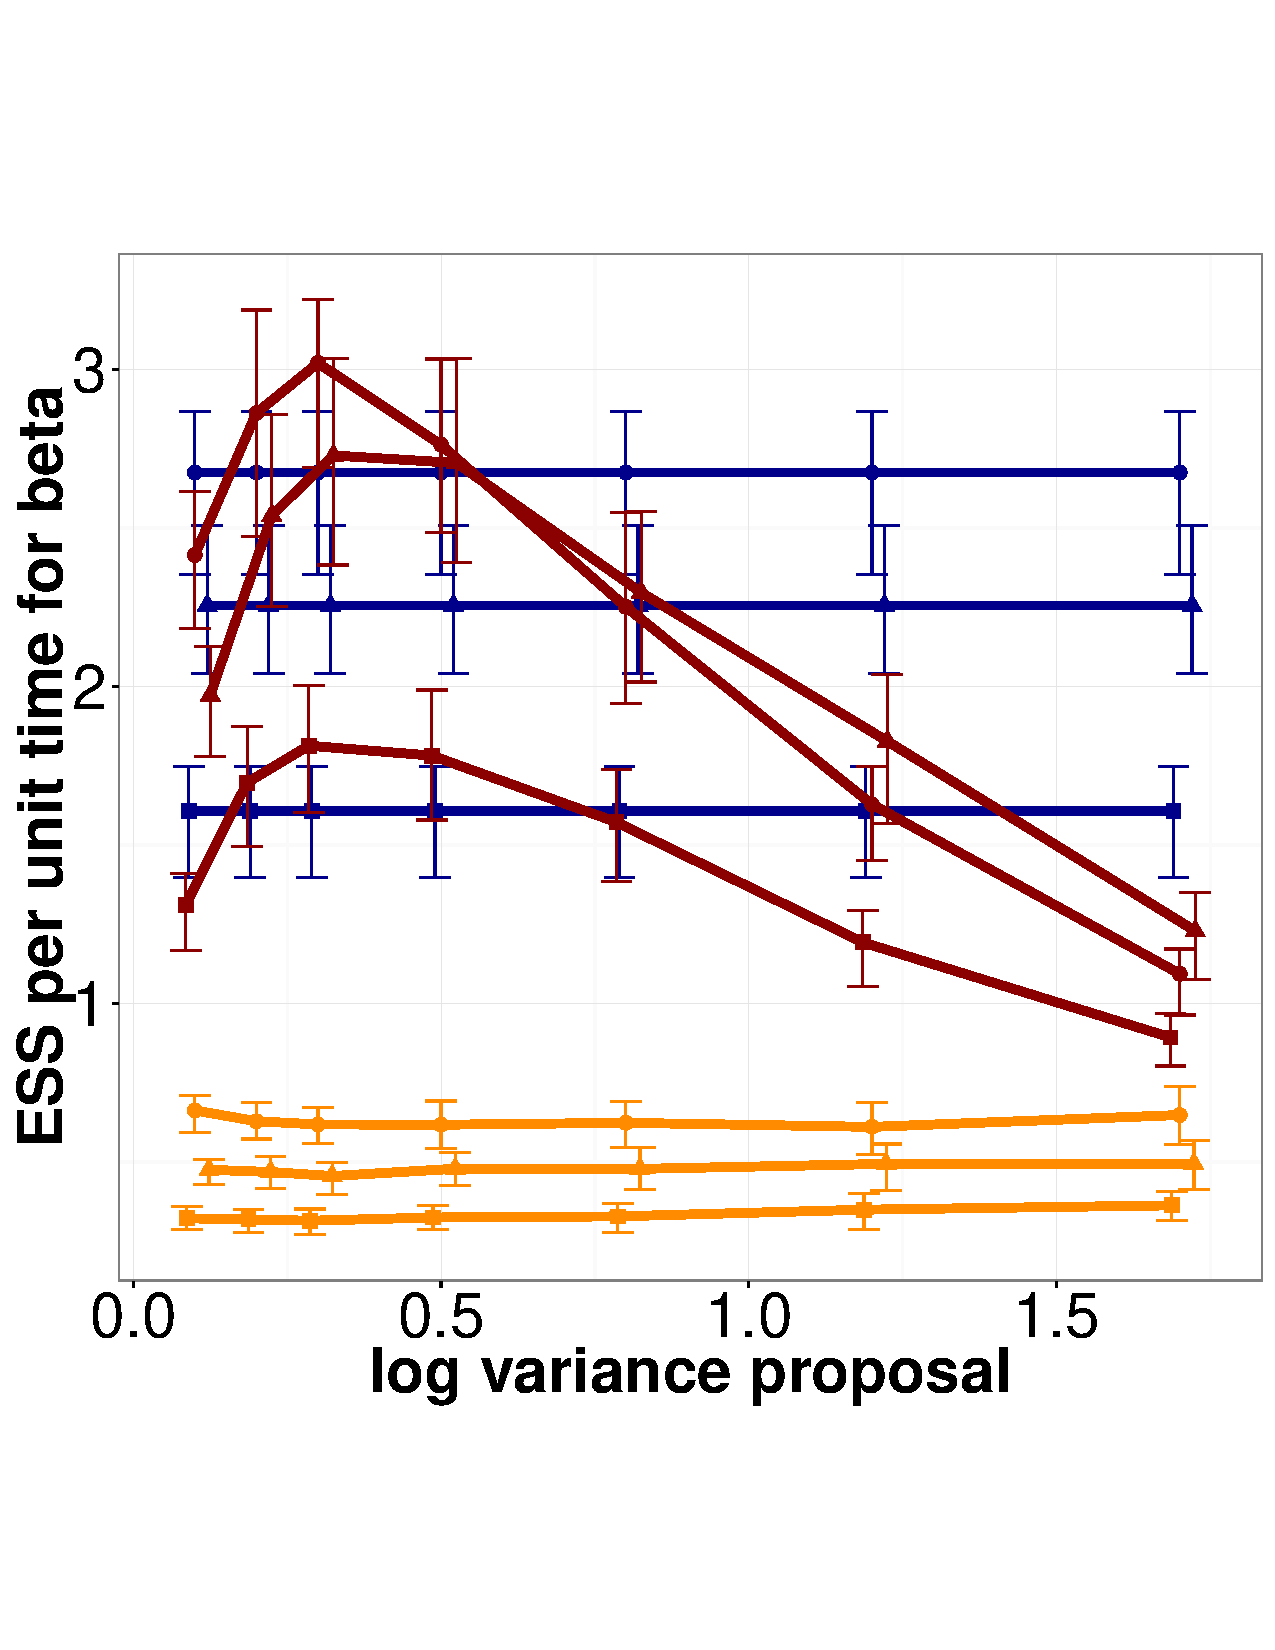
\includegraphics [width=0.44\textwidth, angle=0]{figs/q_5_beta.pdf}
  \end{minipage}
  \begin{minipage}[!hp]{0.33\linewidth}
    \caption{ESS/sec for the immigration model, with dimension 5. (Left, 
      right) are $(\alpha, \beta)$. Red, yellow, and blue curves are the symmetrized MH,
  \naive\ MH, Gibbs sampling and particle MCMC.}
     \label{fig:ESS_Q_D5}
  \end{minipage}
  \centering
  \begin{minipage}[!hp]{0.65\linewidth}
  \centering
    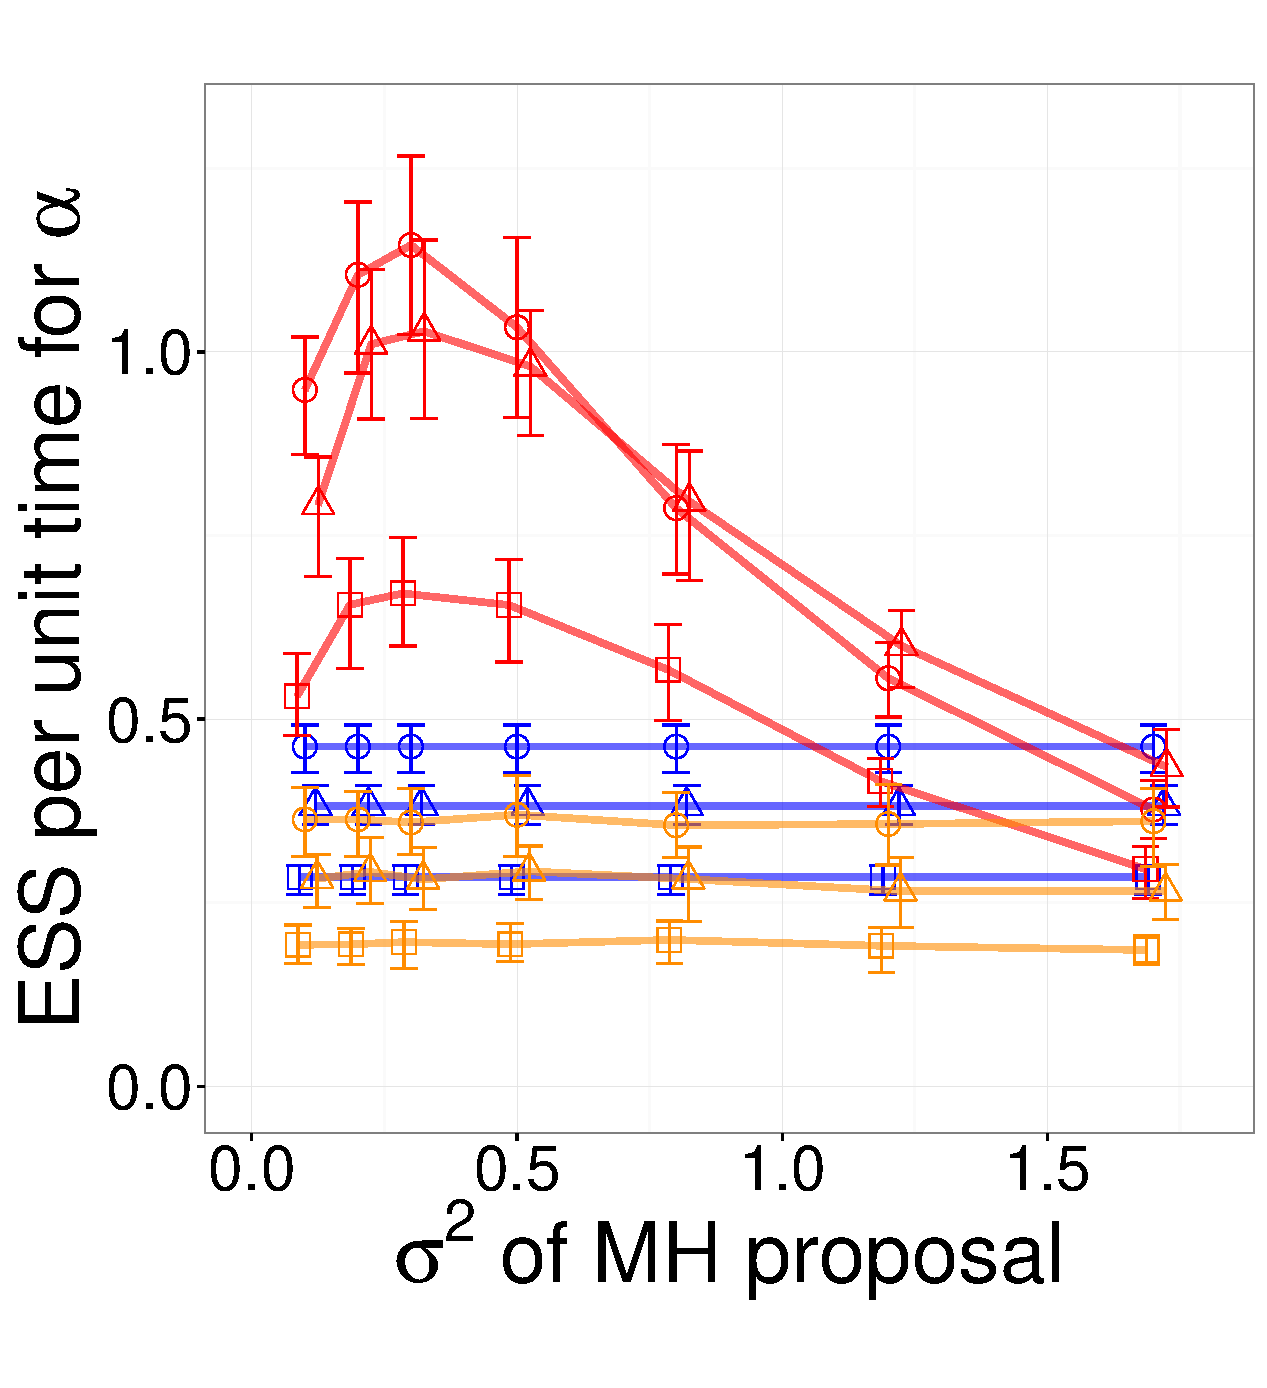
\includegraphics [width=0.44\textwidth, angle=0]{figs/pc_5_alpha.pdf}
    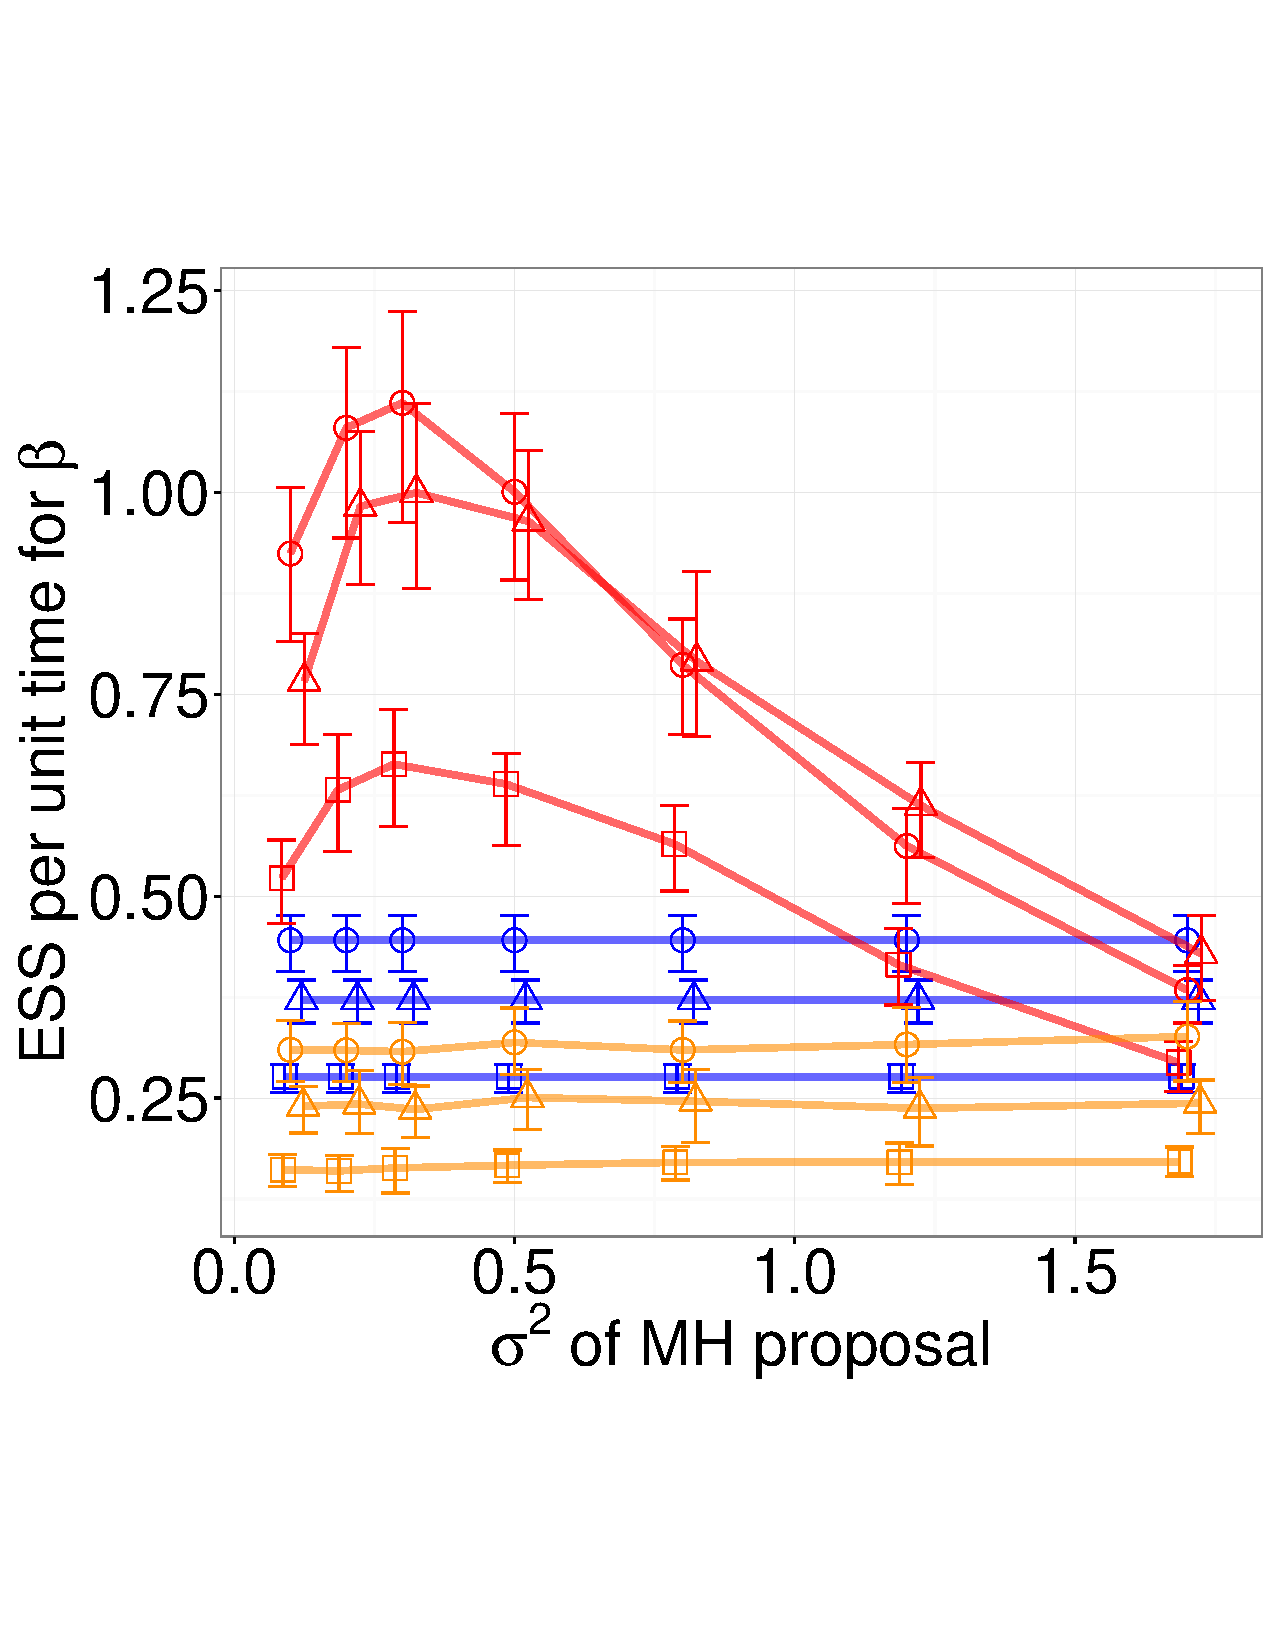
\includegraphics [width=0.44\textwidth, angle=0]{figs/pc_5_beta.pdf}
  \end{minipage}
  \begin{minipage}[!hp]{0.33\linewidth}
    \caption{ESS/sec for the time-inhomogeneous immigration model, with 
      dimension 5. (Left, right) are $(\alpha, \beta)$. Red, yellow and blue curves are the symmetrized MH,
  \naive\ MH, and Gibbs algorithm.}
     \label{fig:ESS_pc_5}
  \end{minipage}
% \centering
% \begin{minipage}[!hp]{0.64\linewidth}
%   \hspace{.15in}
%   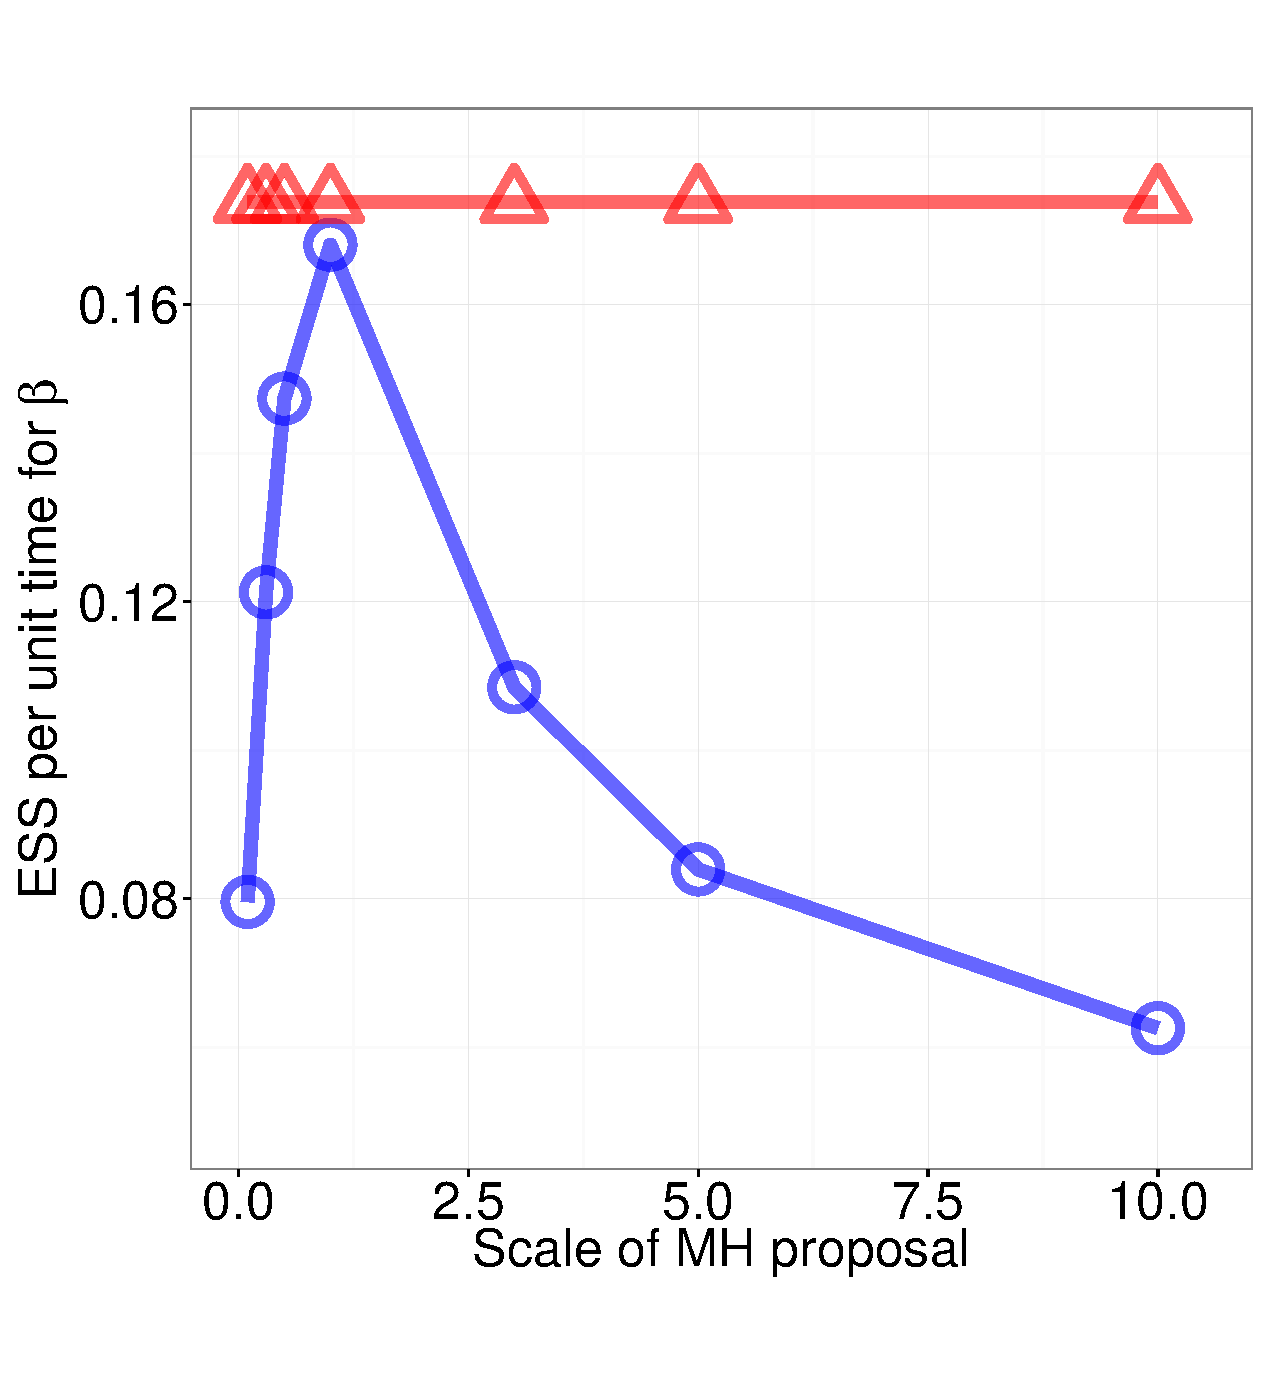
\includegraphics [width=0.44\textwidth, angle=0]{figs/ECOLI_beta.pdf}
%   \hspace{.15in}
%   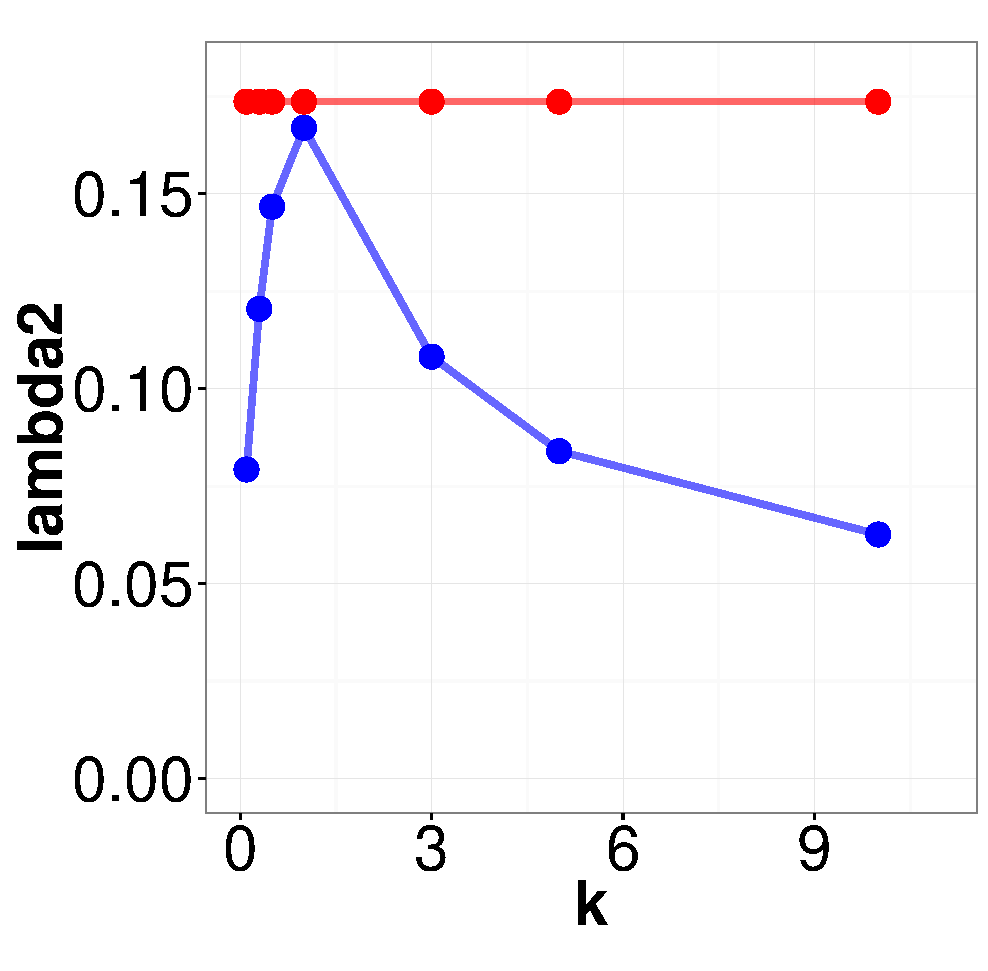
\includegraphics [width=0.44\textwidth, angle=0]{figs/ECOLI_l2.pdf}
% \end{minipage}
%   \hspace{-.3in}
% \begin{minipage}[!hp]{0.05\linewidth}
%   \hspace{0in}
%   \end{minipage}
% \begin{minipage}[!hp]{0.33\linewidth}
%   \caption{ESS/sec for EColi data. The left column is for $\beta$, and the 
%   right is for $\lambda_2$. Red and blue curves are Gibbs algorithm and the symmetrized MH.}
% \end{minipage}
%    \label{fig:ECOLI_beta_l2}
  \end{figure}
  \begin{figure}[H]
%    \vspace{-.2in}
  \centering

  \begin{minipage}[!hp]{0.99\linewidth}
    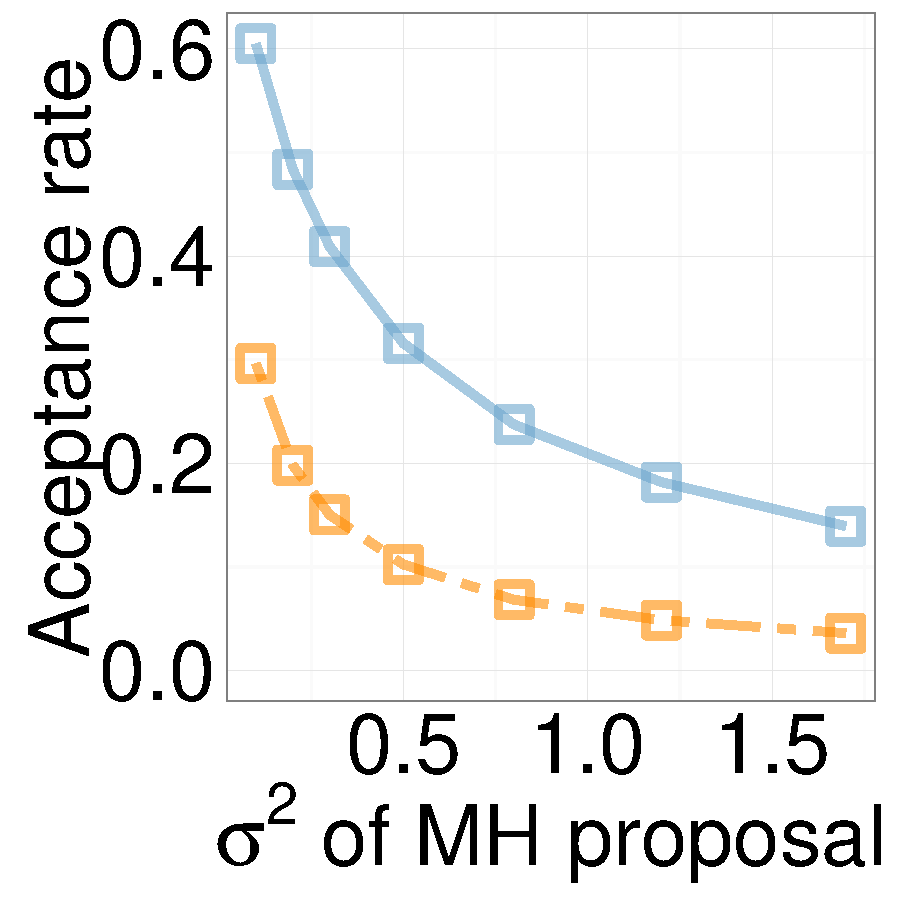
\includegraphics [width=0.40\textwidth, angle=0]{figs/acc/Q_D3alpha_k2.pdf}
	\hspace{.5in}
    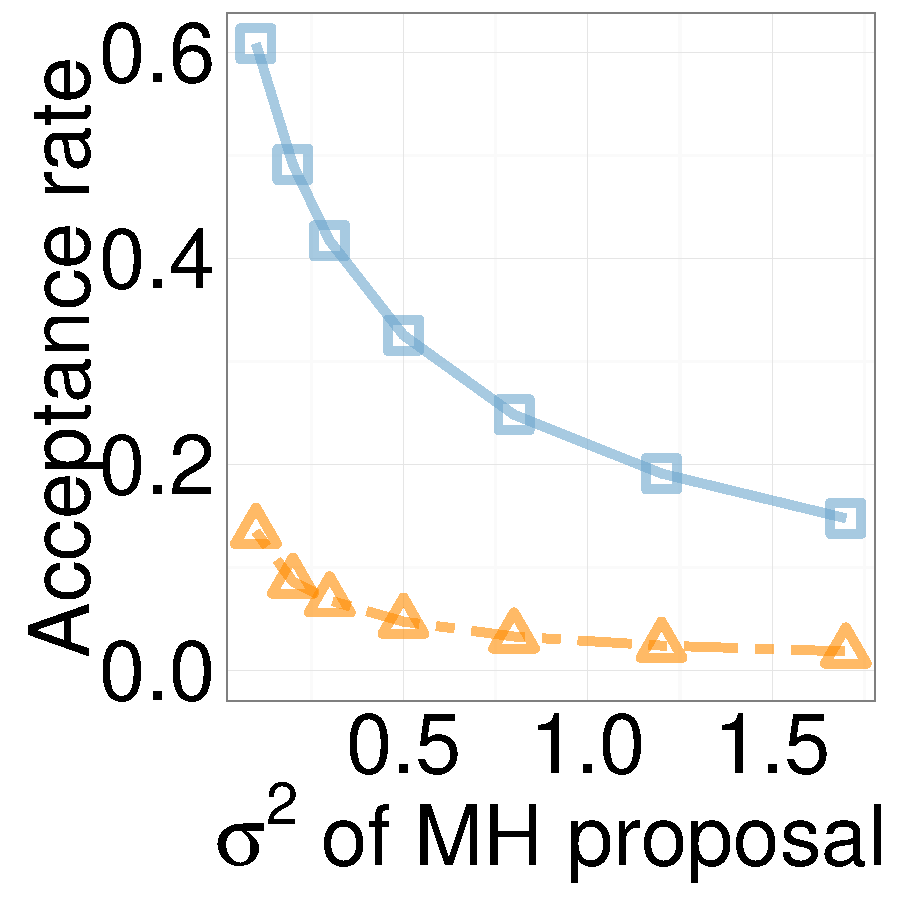
\includegraphics [width=0.40\textwidth, angle=0]{figs/acc/Q_D10alpha_k2.pdf}
  \end{minipage}
%  \begin{minipage}[!hp]{0.99\linewidth}
    \caption{Acceptance Rate for $\alpha$ in the synthetic model, the left row being dimension 3, and the right,dimension 10.  Yellow and blue curves represent symmetrized MH,
 and \naive\ MH  algorithm. The multiplicative factor is $2$. }
     \label{fig:ACC_Q}
%  \end{minipage}
  \end{figure}

%%%% Time-homog
%    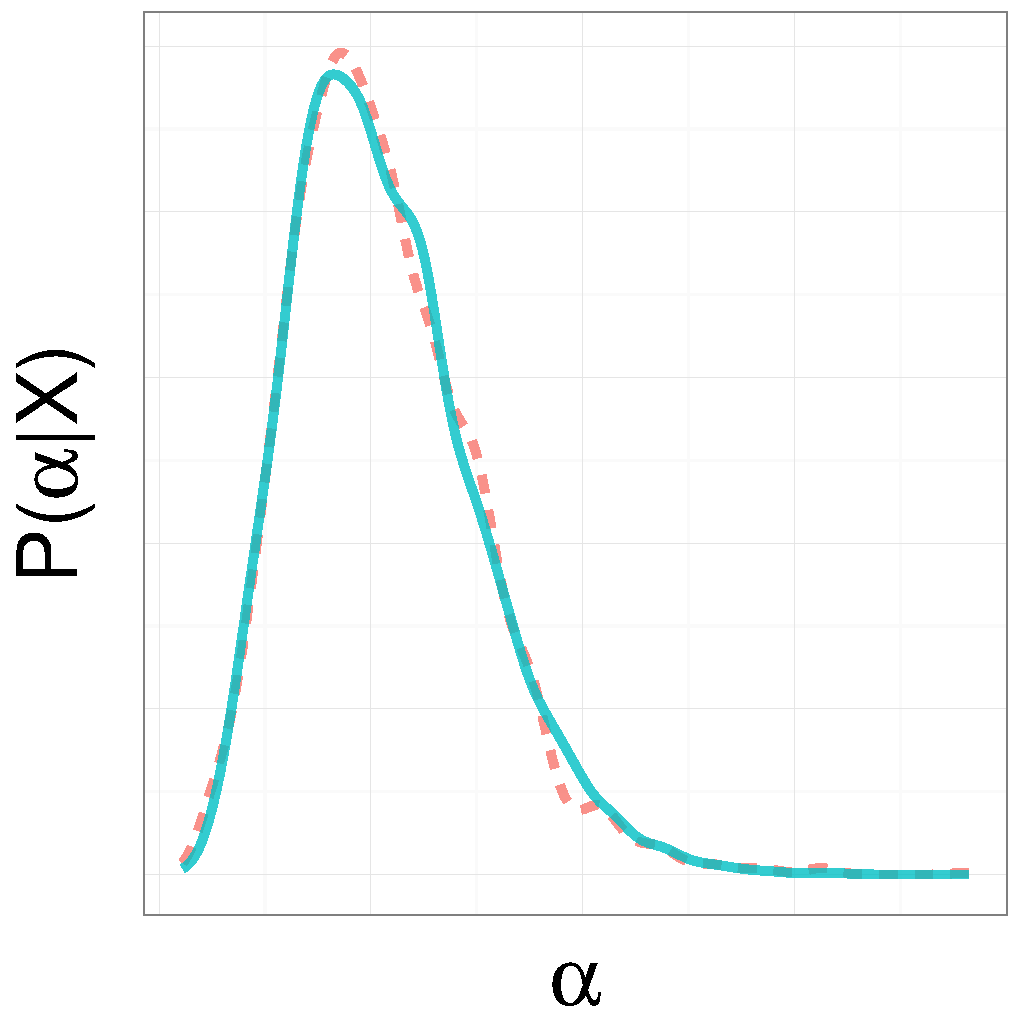
\includegraphics [width=0.19\textwidth, angle=0]{figs/Q_ks/q_hist_20_03_3_.pdf}
%%%%%%%%

  \begin{figure}[H]
%    \vspace{-.2in}
  \centering

  \begin{minipage}[!hp]{0.99\linewidth}
    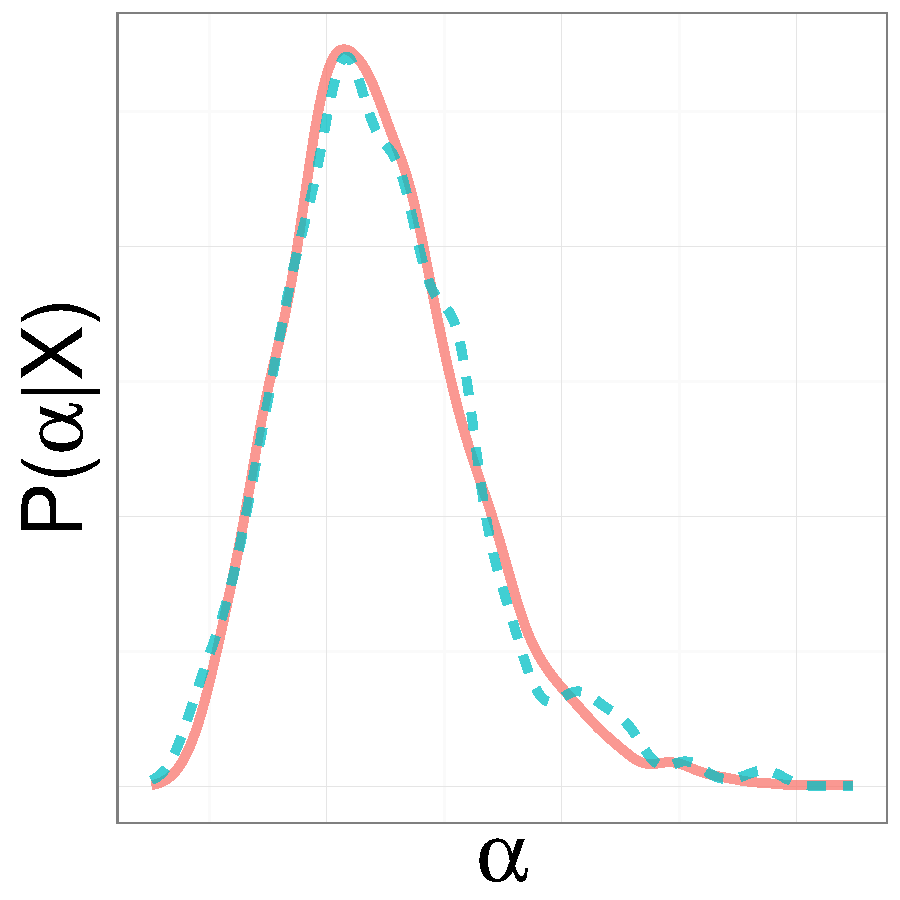
\includegraphics [width=0.3\textwidth, angle=0]{figs/QC_ks/qc_hist_4_03_10_.pdf}
    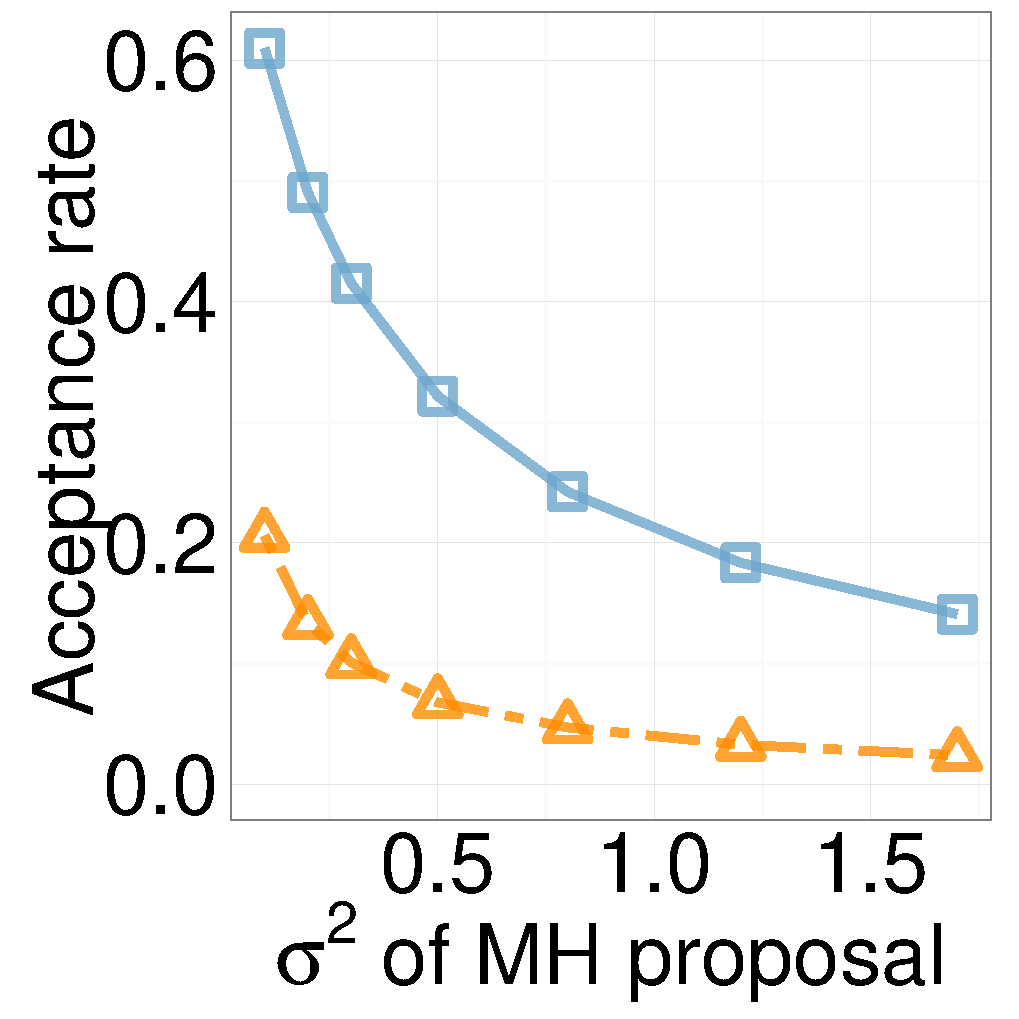
\includegraphics [width=0.30\textwidth, angle=0]{figs/acc/CQ_D3alpha_k2.pdf}
	\hspace{.5in}
    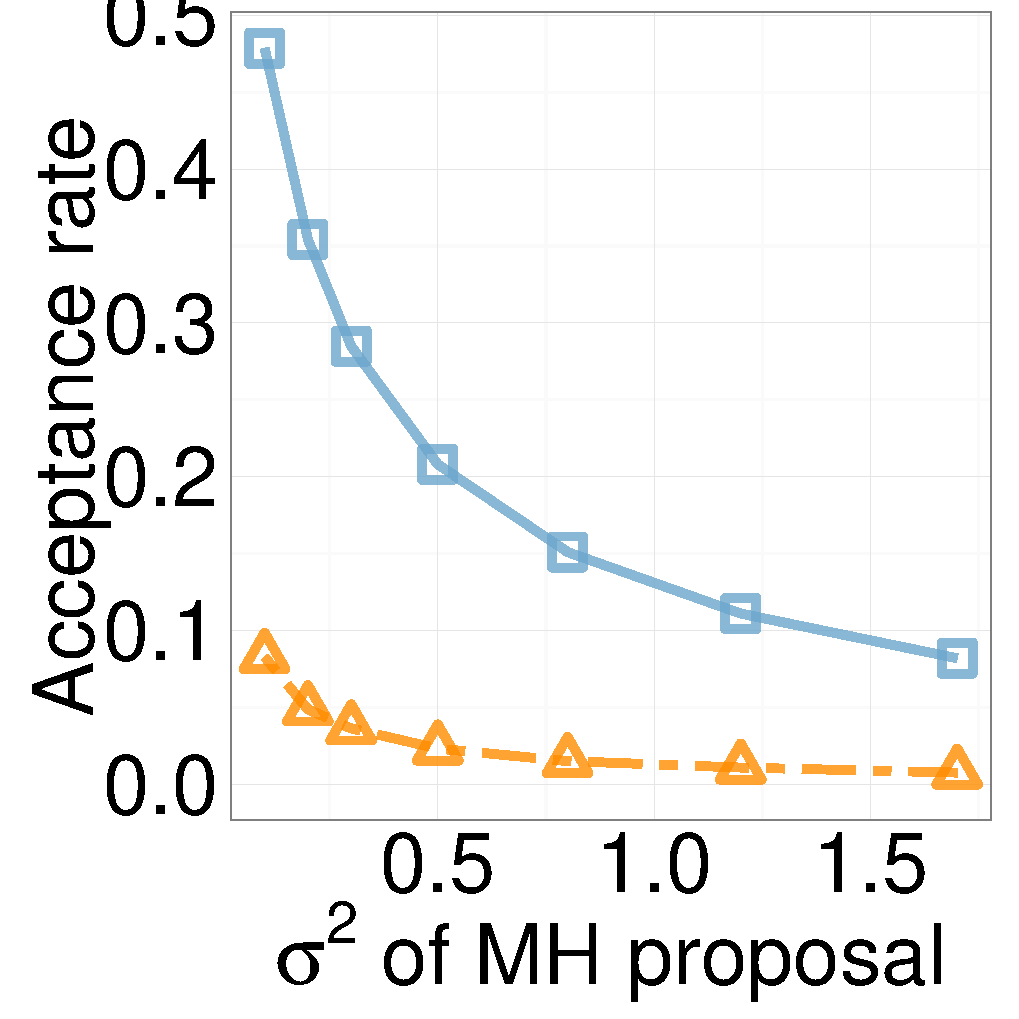
\includegraphics [width=0.30\textwidth, angle=0]{figs/acc/CQ_D10alpha_k2.pdf}
  \end{minipage}
%  \begin{minipage}[!hp]{0.99\linewidth}
    \caption{Acceptance Rate for $\alpha$ in the time-inhomogeneous immigration model, the left row being dimension 3, and the right,dimension 10.  Yellow and blue curves represent symmetrized MH,
 and \naive\ MH  algorithm. The multiplicative factor is $2$. }
     \label{fig:ACC_CQ}
%  \end{minipage}
  \end{figure}

  \begin{figure}[H]
%    \vspace{-.2in}
  \centering

  \begin{minipage}[!hp]{0.99\linewidth}
	\centering
    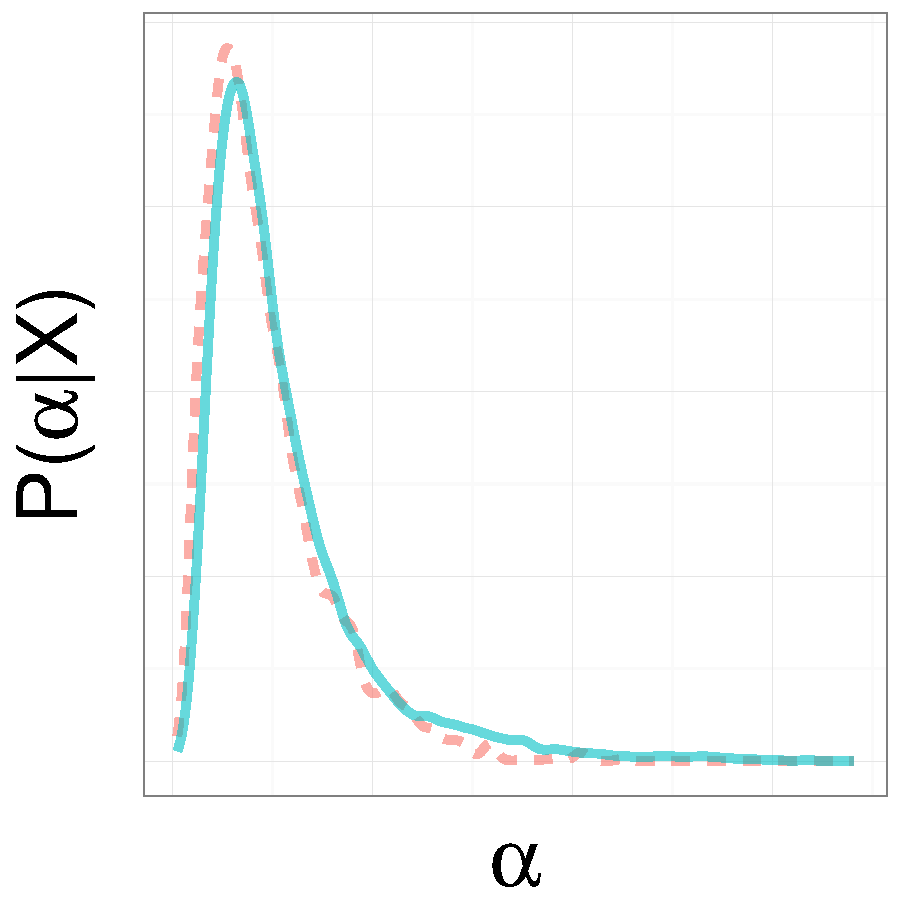
\includegraphics [width=0.3\textwidth, angle=0]{figs/ecoli_ks/ecoli_alphahist_31_3_0_.pdf}
    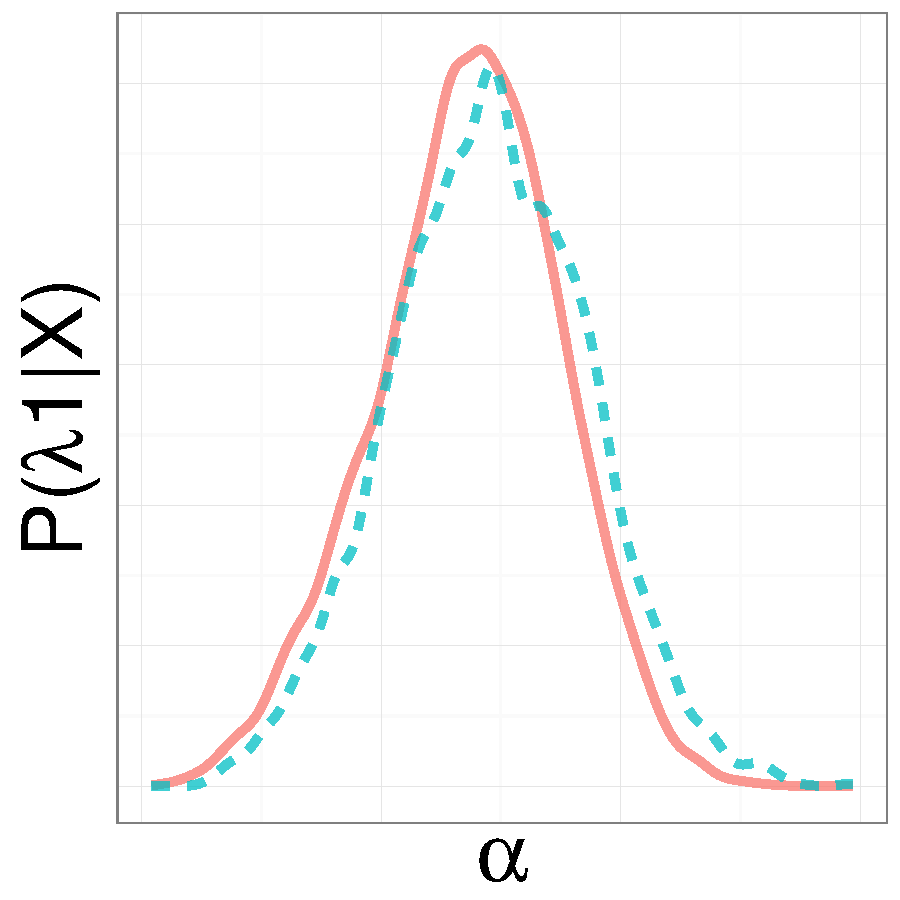
\includegraphics [width=0.3\textwidth, angle=0]{figs/ecoli_ks/ecoli_l1hist_31_3_0_.pdf}
    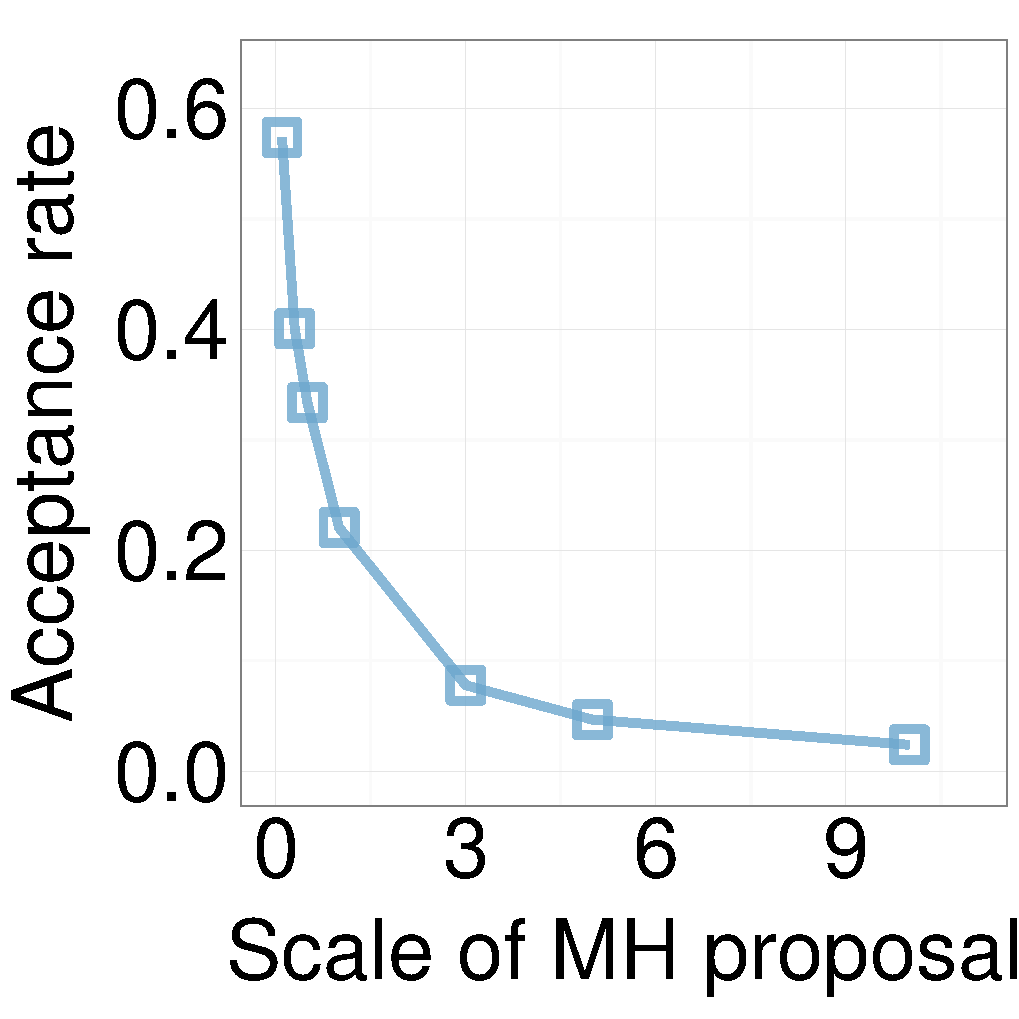
\includegraphics [width=0.30\textwidth, angle=0]{figs/acc/ecolialpha_k2.pdf}
  \end{minipage}
%  \begin{minipage}[!hp]{0.99\linewidth}
    \caption{Acceptance Rate of $\alpha$ generated by the symmetrized MH algorithm for the E.\ Coli data . The multiplicative factor is $2$. }
     \label{fig:ACC_ECOLI}
%  \end{minipage}
  \end{figure}
